\documentclass[a4paper,DIV=14,twoside,open=right,pdftex,10pt]{scrreprt}
\usepackage[utf8]{inputenc}
\usepackage[T1]{fontenc}
\usepackage{lmodern}
\usepackage{natbib}
	\setcitestyle{square}
\usepackage[french]{babel}
\usepackage{amsmath}
\usepackage[misc,geometry]{ifsym} 
\usepackage{siunitx}
\usepackage{graphicx}
\usepackage{wasysym}
\usepackage{nicefrac}
\usepackage{mathrsfs}

\usepackage{amsthm}
\usepackage{amssymb}
\usepackage{amsfonts}
	\newtheorem{theorem}{Théorème}
\usepackage{stmaryrd}
\usepackage{mathtools}

\usepackage{pgfplots}
	\tikzset{
		every picture/.style={
			execute at begin picture={
   				\shorthandoff{:;!?};
   			}
		},
	}	
\usepackage{tikz-3dplot}
	\tdplotsetmaincoords{60}{110}
	

\usetikzlibrary{calc,patterns,angles,quotes}
\usetikzlibrary{shapes.misc}


\pgfplotsset{compat=1.11}	
\tikzset{font=\footnotesize}		
\usepgfplotslibrary{groupplots}
\usepgfplotslibrary{polar}
\usetikzlibrary{spy}
\usetikzlibrary{positioning}
\usepackage{xstring}
\usepackage{enumitem}
	\newcommand\litem[1]{\item{\bfseries #1\\}}
\usepackage{ccicons}
\usepackage{xspace}

\usepackage[normalem]{ulem}

\usepackage{calc}
\newlength{\depthofsumsign}
\setlength{\depthofsumsign}{\depthof{$\sum$}}
\newlength{\totalheightofsumsign}
\newlength{\heightanddepthofargument}
	
	
\usepackage[singlelinecheck=off,justification=centering]{subcaption}
\newcommand{\mysubfig}[2]{%
	\subcaptionbox{\label{#1}}{%
		\centering
		#2
	}
}
\usepackage{multirow}
\usepackage{titling}
%\usepackage{authblk}
\usepackage{eso-pic}
\usepackage{wrapfig}
\usepackage{cancel}

\usepackage{framed}

\usepackage{etoolbox}
\makeatletter
\patchcmd{\@maketitle}{\LARGE \@title}{\fontsize{16}{19.2}\selectfont\@title}{}{}
\makeatother

%\usepackage{fixltx2e}
\MakeRobust{\overrightarrow}

\usepackage{ifthen}
\def\ChoixDeVersion{prof} 

\usepackage{xparse}


\newcommand{\vect}[1]{\ensuremath{\overrightarrow{#1}}}

\newcommand{\R}[2]{%
	\glsdisp{Resu}{\vect{R}}\left(#1\rightarrow#2\right)
}
\newcommand{\Rc}{\gls{Rc}}

\newcommand{\M}[3]{%
	\glsdisp{Mome}{\vect{M}}_{#1}\left(#2\rightarrow#3\right)
}
\newcommand{\V}[3][\Rc]{%
	\glsdisp{V}{%
		\vect{V}}\left(\nicefrac{#2\in#3}{#1}\right)
}
\newcommand{\G}[3][\Rc]{%
	\glsdisp{G}{%
		\vect{\Gamma}}\left(\nicefrac{#2\in#3}{#1}\right)
}
\newcommand{\Om}[2][\Rc]{%
	\glsdisp{Omega}{%
		\vect{\Omega}\left(\nicefrac{#2}{#1}\right)
	}
}
\newcommand{\diff}[2][\Rc_0]{%
	\left.\frac{\mathrm{d}#2}{\mathrm{d}t}\right|_{#1}
}
\newcommand{\mcin}[3][\Rc]{%
	\glsdisp{sigma}{%
		\vect{\sigma}}_{#2}\left(\nicefrac{#3}{#1}\right)
}
\newcommand{\mdyn}[3][\Rc]{%
	\glsdisp{delta}{%
		\vect{\delta}}_{#2}\left(\nicefrac{#3}{#1}\right)
}

\newcommand{\Ec}[2][\Rc_0]{%
	\glsdisp{Ec}{%
		E_{\mathrm{c}}}\left(\nicefrac{#2}{#1}\right)
}
\newcommand{\torseur}[2]{%
	\left\lbrace\mathscr{#1}\left(#2\right)\right\rbrace
}
\newcommand{\tf}[2]{%
	\torseur{\glsdisp{tf}{F}}{#1\rightarrow #2}
}
\newcommand{\tv}[2][\Rc]{%
	\torseur{\glsdisp{tv}{V}}{\nicefrac{#2}{#1}}
}
\newcommand{\tc}[2][\Rc]{%
	\torseur{\glsdisp{tc}{C}}{\nicefrac{#2}{#1}}
}
\newcommand{\td}[2][\Rc]{%
	\torseur{\glsdisp{td}{D}}{\nicefrac{#2}{#1}}
}

\newcommand{\coords}[4][\Rc]{%
	\prescript{}{#1}{
		\left|
			\begin{array}{l}
				#2\\
				#3\\
				#4\\
			\end{array}
		\right.
	}
}
\newcommand{\inmat}[2][O]{%
	\glsdisp{inmat}{
		\uuline{I_{#1}\left(#2\right)}
	}
}
\newcommand{\incomp}[7][\Rc]{%
	\begin{bmatrix}
		#2		& -#7	& -#6\\
		-#7		& #3	& -#5\\
		-#6		& -#5	& #4	
	\end{bmatrix}_{#1}
}
\newcommand{\inope}[3][O]{%
	\glsdisp{inope}{%
		\vect{\mathcal{I}}_{#1}\left(#2,#3\right)
	}
}
\newcommand{\ints}[2][S]{%
	\int_{P\in #1}#2\mathrm{d}m
}

\newcommand{\puiss}[3][\Rc]{%
	\glsdisp{P}{\mathcal{P}}\left(#2\rightarrow\nicefrac{#3}{#1}\right)
}

\newcommand{\puissm}[2]{%
	\glsdisp{Pm}{\mathcal{P}}\left(#1\rightarrow #1\right)
}


\newcommand{\Ep}[3][\Rc]{%
	\glsdisp{P}{\mathrm{E}_{\mathrm{p}}}\left(#2\rightarrow\nicefrac{#3}{#1}\right)
}

\tikzset{cross/.style={cross out, draw=black, minimum size=2*(#1-\pgflinewidth), inner sep=0pt, outer sep=0pt},
%default radius will be 1pt. 
cross/.default={1pt}}


\newenvironment{note}{
	\itshape
	Note :
}{
}

\newcommand{\dm}{\mathrm{d}m}

\newtheorem{definition}{Définition}
\newcommand\numberthis{\addtocounter{equation}{1}\tag{\theequation}}

\newcommand{\hidden}[1]{%
	\begin{framed}
	\ifthenelse{%
		\equal{\ChoixDeVersion}{prof}
	 }{%
		#1
	 }{%
	 	{\color{white}
	 	#1
	 	}
	 }
	 \end{framed}
}

%\newenvironment{tors}[1]{%
%	\left\lbrace
%		\begin{array}{c}
%}{
%		\end{array}
%	\right\rbrace_{#1}	
%}
\NewDocumentEnvironment{tors}{m}{%
	\left\lbrace
		\begin{array}{c}
}{%
		\end{array}
	\right\rbrace_{#1}	
}
\usepackage[pdfborder={0 0 0},colorlinks=true,linkcolor=blue]{hyperref}
\hypersetup{
    pdfauthor={Dorian Depriester},
    pdfsubject={Support de cours},
    pdftitle={Mécanique Générale},
    pdfkeywords={solide, indéformable, mécanique, dynamique, statique, cinétique, actions, puissance, énergie cinétique}
} 
  
\usepackage[ucmark,toc,acronym]{glossaries}
	\newglossary[nlg]{notation}{not}{ntn}{Notations}
	\loadglsentries{Glossaire}
	\makeglossaries
	\renewcommand{\glspluralsuffix}{}
	\setglossarystyle{index}  

   

\title{Mécanique Générale}
\date{2017}
\author{Dorian \textsc{Depriester}}
%\affil[1]{
%Arts et Métiers ParisTech,

% 2 Cours des Arts et Métiers, 13617 Aix-en-Provence}


%\includeonly{I-Actions}
\begin{document}
	%\maketitle
\begin{titlingpage} %This starts the title page
	\begin{center}
		\begin{LARGE} 
			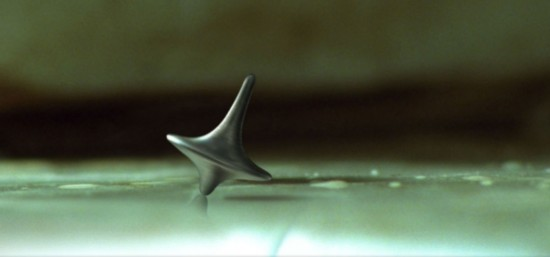
\includegraphics[width=10cm]{Spinning-top-inception}\\
			\vspace{1cm}
			\textbf{\thetitle}\\
		\end{LARGE}
		
		\vspace{3cm}
		\large{\theauthor}\\
		\thedate\\
		\begin{footnotesize}
			Arts et Métiers ParisTech,\\
			2 Cours des Arts et Métiers, 13617 Aix-en-Provence
		\end{footnotesize}
		\vfill
		
\includegraphics[width=5cm]{ENSAM_logo}
	\end{center}
\end{titlingpage}

	\addcontentsline{toc}{chapter}{Table des matières}
	\tableofcontents
	\printglossary[type=notation, title={Liste des symboles}, toctitle={Liste des symboles}]	
%	\listoffigures
%	\listoftables
	

	\chapter{Rappel : éléments de calcul vectoriel}
\section{Produit vectoriel}
	\subsection{Définition}
		\label{sec:def-prodvect}
		\begin{definition}
		Soient \vect{u} et \vect{v} deux vecteurs. On notera $\vect{u}\wedge\vect{v}$ le produit vectoriel de \vect{u} et \vect{v}.
		
%	\subsection{Propriétés}
	Soit \vect{w} un vecteur tel que $\vect{u}\wedge\vect{v}=\vect{w}$. On a alors, par définition du produit vectoriel :
	\begin{itemize}
		\item $\vect{w}$ est orthogonal à $\vect{u}$ et $\vect{v}$,
		\item la base $(\vect{u},\vect{v},\vect{w})$ est directe\footnote{C'est-à-dire qu'elle respecte la règle dite \og des trois doigts de la main droite \fg{}.},
		\item $||\vect{w}||=||\vect{u}||\cdot||\vect{v}||\cdot|\sin(\vect{u},\vect{v})|$.
	\end{itemize}
	\end{definition}
La figure~\ref{fig:produit-vect} illustre ces propriétés.	
	
	\begin{figure}[htbp]
		\centering
		\tdplotsetmaincoords{70}{130}
		\begin{tikzpicture}[tdplot_main_coords,scale=3]
			\draw[,thick,-latex,red] (0,0,0) --(0.7,0,0) node[anchor=north east]{$\vect{u}$};
			\draw[,thick,-latex,blue] (0,0,0) --(0,1.4,0) node[anchor=west]{$\vect{v}$};
			\draw[,thick,-latex,green] (0,0,0) --(0,0,0.98) node[anchor=west]{$\vect{u}\wedge\vect{v}$};
			\tdplotdrawarc[,-stealth]{(0,0,0)}{0.3}{0}{90}{anchor=north}{+}	
			\tdplotsetrotatedcoords{0}{0}{0}
			\tdplotsetrotatedthetaplanecoords{0}	
			\tdplotdrawarc[tdplot_rotated_coords,-stealth]{(0,0,0)}{0.3}{0}{90}{anchor=east}{+}										
			\tdplotsetrotatedthetaplanecoords{90}	
			\tdplotdrawarc[tdplot_rotated_coords,stealth-]{(0,0,0)}{0.3}{0}{90}{anchor=west}{+}	
		\end{tikzpicture}
		\caption{Représentation 3D du produit vectoriel.}
		\label{fig:produit-vect}
	\end{figure}
	D'après la définition précédente, $\vect{u}\wedge\vect{v}=\vect{0}$ si et seulement si $\vect{u}$ et $\vect{v}$ sont colinéaires\footnote{Si l'un des vecteurs est nul, alors il est colinéaire à l'autre.}.
	
	\subsection{Propriétés}
	Le produit vectoriel respecte les propriétés suivantes :
	\begin{itemize}
		\item Il est distributif sur l'addition :
			\begin{equation}
				\left(\vect{u}+\vect{v}\right)\wedge\vect{w}=\vect{u}\wedge\vect{w}+\vect{v}\wedge\vect{w}
			\end{equation}
		\item Il est compatible avec la multiplication par un scalaire :
			\begin{equation}
				\left(\lambda\vect{u}\right)\wedge\vect{v}=\lambda\left(\vect{u}\wedge\vect{v}\right)
			\end{equation}
		\item Il est antisymétrique :
			\begin{equation}
				\vect{u}\wedge\vect{v}=-\vect{v}\wedge\vect{u}
			\end{equation}
	\end{itemize}
	
	\subsection{Calcul}
		Soient deux vecteurs \vect{u} et \vect{v} de coordonnées suivantes :
		\begin{equation}
			\vect{u}
			\left|
			\begin{array}{c}
				u_x\\
				u_y\\
				u_z\\
			\end{array}
			\right.
			\quad
			\text{et }
			\vect{v}
			\left|
			\begin{array}{c}
				v_x\\
				v_y\\
				v_z\\
			\end{array}
			\right.
			\,.		
		\end{equation}
Si $\vect{w}=\vect{u}\wedge\vect{v}$, on a alors :
\begin{equation}
			\vect{w}
			\left|
			\begin{array}{c}
				u_yv_z-v_yu_z\\
				u_zv_x-v_zu_x\\
				u_xv_y-v_xu_y\\
			\end{array}
			\right.
\end{equation}

\section{Extension : produit mixte}
	\subsection{Définition}
		\begin{definition}
			Soient \vect{u}, \vect{v} et \vect{w} trois vecteurs. On note $[\vect{u}, \vect{v}, \vect{w}]$ le scalaire, appelé produit mixte de \vect{u}, \vect{v} et \vect{w}, tel que :
			\begin{equation}
				[\vect{u}, \vect{v}, \vect{w}]=\left(\vect{u}\wedge\vect{v}\right)\cdot\vect{w}
			\end{equation}
			où $\cdot$ est le produit scalaire.
		\end{definition}
		
	\subsection{Propriétés}
		\label{sec:props-prodmixte}
		Outre ses propriétés de linéarité, qui découlent directement de celles du produit vectoriel, le produit mixte respecte les propriétés suivantes :
		\begin{itemize}
			\item Il est identique par permutation circulaire :
			\begin{equation}
				[\vect{u}, \vect{v}, \vect{w}]=[\vect{v}, \vect{w},\vect{u}]=[\vect{w},\vect{u}, \vect{v}]
			\end{equation}
			\item Il est anticommutatif :
			\begin{equation}
				[\vect{u}, \vect{v}, \vect{w}]=-[\vect{v},\vect{u},\vect{w}]=-[\vect{w},\vect{v}, \vect{u}]=-[\vect{u}, \vect{w}, \vect{v}]
			\end{equation}			
		\end{itemize}
		
		
\section{Torseur}
	\subsection{Champ de vecteurs équiprojectif}
On considère un champ de vecteur de l'espace $E$. On note $\vect{M}_X$ la valeur de ce champ au point $X$. Le champ est alors un champ de moment si et seulement si il est équiprojectif, c'est-à-dire si :
\begin{equation}
	\forall A\in E\quad \forall B\in E \quad \vect{M}_A\cdot\vect{AB}=\vect{M}_B\cdot\vect{AB}
\end{equation}
Une illustration de cette propriété est donnée en figure~\ref{fig:equiprojectivite}

\begin{figure}[htbp]
	\centering
	\begin{tikzpicture}
		\begin{axis}[xmin=0.5,xmax=4,ymin=0.5,ymax=3, view={0}{90},ticks=none]
			\addplot3[thin, blue, quiver={u={2.5-0.5*y}, v={0.5*x}, scale arrows=0.3}, -stealth,samples=20] {0};
			\coordinate (A) at (axis cs:1,1);
			\coordinate (Ma) at (axis cs:1.6,1.150);
			\coordinate (B) at (axis cs:3,2);
			\coordinate (Mb) at (axis cs:3.4,2.5);
			\draw[thick] (A) -- (B) node[pos=0,anchor=east]{$A$} node[pos=1,anchor=north]{$B$};
			\draw[thick,red,-stealth] (A) -- (Ma);
			\draw[thick,red,-stealth] (B) -- (Mb);
			\draw[red] (A) -- (axis cs: 1+0.27*2,1+0.27) -- (Ma);
			\draw[red] (A) -- (axis cs: 3+0.27*2,2+0.27) -- (Mb);
		\end{axis}
	\end{tikzpicture}
	\caption{Représentation d'un champ de vecteurs équiprojectif (flèches) : la projection sur le segment $AB$ de la valeur du champ en $A$ est identique à la projection sur ce même segment de la valeur du champ en $B$.}
	\label{fig:equiprojectivite}
\end{figure}

	\subsection{\'Elements de réduction d'un torseur}
	Un torseur est un object mathématique constitué :
	\begin{itemize}
		\item d'un vecteur, appelé résultante
		\item d'un champ de moment
	\end{itemize}
	
	Comme le champ de moment respecte la formule du champ de moment (voir ci-après), la connaissance de la valeur de ce champ en un point suffit à déterminer la valeur du champ en tout point de l'espace. Soient \vect{R} la résultante et $\vect{M}_A$ le moment en $A$ du torseur $\lbrace\mathcal{T}\rbrace$. Ce dernier peut alors s'écrire sous la forme suivante :
	\begin{equation}
		\left\lbrace\mathcal{T}\right\rbrace=\left\lbrace\begin{array}{c}
			\vect{R}\\
			\vect{M}_A
		\end{array}\right\rbrace_A
	\end{equation}
	\vect{R} et $\vect{M}_A$ sont les éléments de réduction du torseur.
	
	\subsection{Champ de moments de torseur}
		\label{sec:champ-de-moments}
		La valeur du moment en tout point $B$ de l'espace $E$, notée $\vect{M}_B$, peut se calculer ainsi :
		\begin{equation}
			\label{eq:champ-de-moments}
			\forall B\in E \quad \vect{M}_B=\vect{M}_A+\vect{BA}\wedge\vect{R}
		\end{equation}
		
	\subsection{Axe central d'un torseur}
		\label{sec:axe-central}
		On appelle axe central d'un torseur l'ensemble des points où la norme du moment est minimale. Cet axe est aussi caractérisé par le fait que résultante et moment y sont colinéaires.
		
		
	\subsection{Opérations entre torseurs}
		Soient deux torseurs $\lbrace\mathcal{T}\rbrace$ et $\lbrace\mathcal{T}'\rbrace$ avec :
		\begin{equation}
			\left\lbrace\mathcal{T}\right\rbrace=\left\lbrace\begin{array}{c}
				\vect{R}\\
				\vect{M}_A
			\end{array}\right\rbrace_A
			\quad
			\text{et}
			\quad
			\left\lbrace\mathcal{T}'\right\rbrace=\left\lbrace\begin{array}{c}
				\vect{R}'\\
				\vect{M}_A'
			\end{array}\right\rbrace_A					
		\end{equation}

		\subsubsection{Somme}
		La somme de deux torseurs se calcule comme la somme de ses éléments de réduction, calculés en un même point :
		\begin{equation}
			\left\lbrace\mathcal{T}\right\rbrace+\left\lbrace\mathcal{T}'\right\rbrace=
			\left\lbrace\begin{array}{c}
				\vect{R}+\vect{R}'\\
				\vect{M}_A+\vect{M}_A'
			\end{array}\right\rbrace_A			
		\end{equation}
		
		\subsubsection{Produit}
			\label{sec:produit-torseurs}
		Le produit de deux torseurs se calcule comme la somme des produits croisés de leurs éléments de réduction, calculés en un même point :
		\begin{equation}
			\left\lbrace\mathcal{T}\right\rbrace\cdot\left\lbrace\mathcal{T}'\right\rbrace=
				\vect{R}\cdot\vect{M}_A'+\vect{M}_A\cdot\vect{R}'
		\end{equation}
		Cette somme est indépendante du point auquel sont calculés les moments.	
		
		\subsubsection{Égalité}
		Deux torseurs sont égaux si et seulement si leurs éléments de réductions, calculés au même point, sont égaux deux à deux :
		\begin{equation}
			\left\lbrace\mathcal{T}\right\rbrace=\left\lbrace\mathcal{T}'\right\rbrace
			\quad\Leftrightarrow\quad
			\left\lbrace
				\begin{aligned}
					\vect{R}&=\vect{R}'\\
					\vect{M}_A&=\vect{M}_A'
				\end{aligned}
			\right\rbrace
		\end{equation}	
		


	\chapter{Modélisation des actions entre solides}
	\section{Torseur des actions mécaniques}
		\subsection{Définition}
					
\begin{wrapfigure}{l}{0.4\textwidth}
	\centering
	\begin{tikzpicture}[scale=0.7]
		\draw[red] (0,0) ellipse (2 and 1);
		\node at (0,0) {$(1)$};
		\draw[blue] (4.5,0) ellipse (2.5 and 1);
		\node at (4.5,0) {$(2)$};
		\draw (2,0) -- ++(0.1,0) node[anchor=west]{$A$};
		\draw (2,0) -- ++(-0.1,0);
	\end{tikzpicture}
\end{wrapfigure}
Soient deux solides $(1)$ et $(2)$, en contact mutuel en $A$. L'action de $(1)$ sur $(2)$ est représenté par le torseur des actions mécaniques suivant :
\medskip
\hidden{
\begin{equation}
	\torseur{F}{1\rightarrow2}=\left\lbrace
		\begin{array}{c}
				\R{1}{2}\\
				\M{A}{1}{2}
		\end{array}
	\right\rbrace_A
\end{equation}
}

$\R{1}{2}$ est la force appliquée par $(1)$ sur $(2)$ tandis que $\M{A}{1}{2}$ est le moment en $A$ de l'effort appliqué par $(1)$ sur $(2)$.

		\subsection{Cas particuliers}
		\begin{itemize}
			\item Si la résultante des efforts de $(1)$ sur $(2)$ est nulle, alors on dit que l'action de $(1)$ sur $(2)$ est un couple pur. Ce couple est constant, d'après la formule du champ de moments de torseur.
			\item Si le moment est nul en un point $A$, alors le torseur est un \emph{glisseur}.
		\end{itemize}
		
		\section{Champ de pesanteur}
		\label{sec:centre-de-masse}
		\subsection{Centre d'inertie}
\begin{definition}
\hidden{
Soit $G$ un point d'un solide $S$. $G$ est d'inertie de $S$ si et seulement si :
	\begin{equation}
		\int_{P\in S}\vect{GP}\dm=\vect{0}
		\label{eq:def-G}
	\end{equation}
}
\end{definition}

\begin{theorem}
\hidden{
	Soit un solide $S$ de masse $m$. Le centre d'inertie $G$ de $S$ vérifie alors :
	\begin{equation}
		\forall A\quad\vect{AG}=\frac{1}{m}\int_{P\in S}\vect{AP}\dm
	\end{equation}	 
}
\end{theorem}

\begin{proof}
	\begin{alignat*}{7}
		&&&\vect{AP}&&=&&\vect{AG}&&+&&\vect{GP}&\\
		&\implies\quad& \int_{P\in S}&\vect{AP}&\dm&=&\int_{P\in S}&\vect{AG}&\dm&+&\int_{P\in S}&\vect{GP}&\dm\\
		&\iff\quad& \int_{P\in S}&\vect{AP}&\dm&=&&\vect{AG}&\int_{P\in S}\dm&+&&\vect{0}&\\
		&\iff\quad& \int_{P\in S}&\vect{AP}&\dm&=&&\vect{AG}m&
	\end{alignat*}
\end{proof}

		\subsection{Actions du champ de pesanteur}

\begin{theorem}
\hidden{
	Soit $S$ un solide de masse $m$ soumis au champ de pesanteur, supposé uniforme et dirigé suivant une direction $-\vect{z}$ : $\vect{g}=-g\vect{z}$. Le torseur des actions de pesanteur s'écrit alors :
	\begin{equation}
		\torseur{F}{g\rightarrow S}=\left\lbrace
			\begin{array}{c}
					-mg\vect{z}\\
					\vect{0}
			\end{array}
		\right\rbrace_G
	\end{equation}
}	
\end{theorem}

\begin{proof}
	Soit un petit élément de masse $\dm$ de $S$. L'action de pesanteur sur cet élément vaut alors :
	\begin{alignat*}{4}
		&&				&\mathrm{d}\R{g}{S}	&=&-\vect{g} \dm&\\
		&\implies\quad&	&\R{g}{S}			&=&\int_{P\in S}\vect{g}\dm&=\int_{P\in S}-g\vect{z}\dm=-g\vect{z}\int_{P\in S}\dm\\
		&\iff\quad&&\R{g}{S}&=&-mg\vect{z}&
	\end{alignat*}
	
	De la même façon, si on calcule le moment en $A$ :
	\begin{equation*}
		\M{A}{g}{S}=\int_{P\in S}\vect{AP}\wedge\left(-g\vect{z}\right)\dm
		=-g\int_{P\in S}\vect{AP}\wedge\vect{z}\dm
		=-g\left(\int_{P\in S}\vect{AP}\dm\right)\wedge\vect{z}
	\end{equation*}
	
Soit $G$ le centre de gravité de $S$. On a alors~\eqref{eq:def-G} :
\begin{equation*}
	\int_{P\in S}\vect{GP}\dm=\vect{0}
\end{equation*}
On a alors :
\begin{equation*}
	\M{G}{g}{S}=\vect{0}
\end{equation*}	
\end{proof}

\section{Actions de contact}
	\subsection{Contact ponctuel}
	\begin{minipage}[b]{0.4\textwidth}
		\begin{tikzpicture}[scale=1.2]
		    \draw (0,0) circle (1cm);
		    \shade[ball color=red!10!white] (0,0) circle (1);
		    \draw[fill=green,opacity=0.5] (-1,2) --++ (-1,-2) node[opacity=1,anchor=south west]{$(\pi)$} --++ (3,0) --++ (+1,+2) -- cycle;
		    \draw (0,2) circle (1cm);
		    \shade[ball color=blue!10!white] (0,2) circle (1);
		    \coordinate (P) at (0,1);
		    \draw (P)--++(0.1,0);
		    \draw (P)--++(-0.1,0);
		    \draw (P)--++(0,0.1);
		    \draw (P)--++(0,-0.1);
		    \node[anchor=north west] at (P){$P$};		
			\node at (0.5,-0.5){$S_1$};    
			\node at (0.5,1.5){$S_2$};
			\draw[-latex,very thin] (P)-- ++ (0,2.3) node[anchor=west]{$\vect{n}$}; 
			\coordinate (Om) at (-0.5,2);
			\coordinate (Pn) at (0,2.2);
			\coordinate (Pp) at (-0.5,0.6);
			\draw[blue,thick,-latex] (P) --(Om) node[anchor=east]{$\R{S_1}{S_2}$};
			\draw[red,very thick,-latex] (P) --(Pn) node[anchor=west]{$\vect{N}$};
			\draw[red,very thick,-latex] (P) --(Pp) node[anchor=north]{$\vect{T}$};
			\draw[very thin, dashed,red] (Pn) -- (Om) -- (Pp);
		\end{tikzpicture}
	\end{minipage}
	\begin{minipage}[b]{0.5\textwidth}
		\begin{theorem}
			Soient deux solides $S_1$ et $S_2$, en contact ponctuel en un point $P$. On note $(\pi)$ le plan tangent à $S_1$ et $S_2$ en $P$. L'action qu'exerce $S_1$ sur $S_2$ peut alors être représentée un glisseur, d'axe central passant par $P$ :
			\begin{equation}
				\tf{S_1}{S_2}=
				\begin{tors}{P}
					\R{S_1}{S_2}\\
					\vect{0}
				\end{tors}					
			\end{equation}
		\end{theorem}
	\end{minipage}
	
		On décompose la résultante comme la somme d'un composante normale à $(\pi)$, notée $\vect{N}$ et d'un composante tangentielle, notée $\vect{T}$ :
		\begin{equation}
			\R{S_1}{S_2}=\vect{N}+\vect{T}
		\end{equation}	
 Si on note $\vect{n}$ la normale à  $(\pi)$, on a donc :
		\begin{subequations}
			\begin{align}
				\vect{N} &\parallel \vect{n}\\
				\vect{T} &\perp \vect{n}
			\end{align}
		\end{subequations}
		
	\subsection{Lois de Coulomb}
		\subsubsection{Glissement}
		\begin{minipage}[b]{0.4\textwidth}
			\begin{tikzpicture}
				\coordinate (s) at (-1.5cm,0);
				\draw[-latex,very thin] (s)-- ++ (0,4) node[anchor=west]{$\vect{n}$} coordinate[pos=0.5] (t);
				\draw[fill=green,opacity=0.5] (-3,0,-1) --++ (3,0,0) node[anchor=north west]{$(\pi)$} --++ (0,0,2) --++ (-3,0,0) -- cycle;
				\fill[opacity=0.1,draw] (0,3) arc (0:180:1.5cm and 0.4cm)coordinate[pos=0] (a);
				\draw (0,3) arc (0:-180:1.5cm and 0.4cm)coordinate (b) coordinate[pos=0.3](P);
				\fill[opacity=0.1,draw] (a) -- (s) -- (b);
				\draw[blue,thick,-latex] (s) -- (P) node[anchor=north west]{$\R{S_1}{S_2}$};
				\node[anchor=north] at (s) {$P$};
				\draw[latex-latex] (t) arc (90:130:1.25) node[midway,anchor=south]{$\varphi$};
				\coordinate (pt) at (-0.3,0,1);
				\coordinate (pn) at (-1.5,3);
				\draw[red,very thick,-latex] (s) --(pt) node[anchor=north]{$\vect{T}$};
				\draw[red,very thick,-latex] (s) --(pn) node[anchor=east]{$\vect{N}$};
				\draw[dashed] (pn) -- (P) -- (pt);
  			\end{tikzpicture}
  		\end{minipage}
		\begin{minipage}[b]{0.5\textwidth}
			\begin{theorem}
				Si les solides $S_1$ et $S_2$ glissent l'un sur l'autre, c'est-à-dire si $\V[S_1]{P}{S_2}\neq\vect{0}$ (cf. \S\ref{sec:glissement} p.\pageref{sec:glissement}), on a alors :
				\begin{equation}
					\lVert \vect{T}\rVert=\mu_{\mathrm{d}}\lVert \vect{N}\rVert
				\end{equation}
				et $\vect{T}$ qui est opposé à la vitesse de glissement $\V[S_1]{P}{S_2}$. $\mu_{\mathrm{d}}$ est le coefficient de frottement dynamique.
			\end{theorem}
			\begin{definition}
				On appelle angle de frottement l'angle $\varphi$ tel que :
				\begin{equation}
					\mu_{\mathrm{d}}=\tan\varphi
				\end{equation}
			\end{definition}
			Lors du glissement, la résultante de l'effort est sur le cône de frottement.
		\end{minipage}
		
	\subsubsection{Adhérence}
		\begin{minipage}[b]{0.4\textwidth}
			\begin{tikzpicture}
				\coordinate (s) at (-1.5cm,0);
				\coordinate (P) at (-0.5,2.9);
				\draw[blue,thick,-latex] (s) -- (P) node[anchor=north west]{$\R{S_1}{S_2}$};
				\draw[-latex,very thin] (s)-- ++ (0,4) node[anchor=west]{$\vect{n}$} coordinate[pos=0.5] (t);
				\draw[fill=green,opacity=0.5] (-3,0,-1) --++ (3,0,0) node[anchor=north west]{$(\pi)$} --++ (0,0,2) --++ (-3,0,0) -- cycle;
				\fill[opacity=0.1,draw] (0,3) arc (0:180:1.5cm and 0.4cm)coordinate[pos=0] (a);
				\draw (0,3) arc (0:-180:1.5cm and 0.4cm)coordinate (b);
				\fill[opacity=0.1,draw] (a) -- (s) -- (b);
				\node[anchor=north] at (s) {$P$};
				\draw[latex-latex] (t) arc (90:130:1.25) node[midway,anchor=south]{$\varphi$};
				\coordinate (pt) at (-0.2,0.1,1);
				\coordinate (pn) at (-1.5,3);
				\draw[red,very thick,-latex] (s) --(pt) node[anchor=north]{$\vect{T}$};
				\draw[red,very thick,-latex] (s) --(pn) node[anchor=east]{$\vect{N}$};
				\draw[dashed] (pn) -- (P) -- (pt);
  			\end{tikzpicture}
  		\end{minipage}
  		\begin{minipage}[b]{0.5\textwidth}
			\begin{theorem}
				Si les solides $S_1$ et $S_2$ ne glissent pas l'un sur l'autre, c'est-à-dire si $\V[S_1]{P}{S_2}=\vect{0}$, on a alors :
				\begin{equation}
					\lVert \vect{T}\rVert<\mu_{\mathrm{s}}\lVert \vect{N}\rVert
				\end{equation}
				avec $\mu_{\mathrm{s}}$ le coefficient de frottement statique.
			\end{theorem}
			Il y a adhérence si la résultante de l'effort est à l'intérieur du cône de frottement.
		\end{minipage}
		
		Généralement, le coefficient de frottement dynamique est plus faible que le coefficient de frottement statique :
		\begin{equation}
			\mu_{\mathrm{d}}\leq\mu_{\mathrm{s}}
		\end{equation}

	\chapter{Cinématique}
	\section{Vecteur position d'un point d'un solide}
	\begin{definition}
	Soient $t$ la variable de temps et $S$ un solide en mouvement par rapport à un repère $\Rc(O,\vect{x},\vect{y},\vect{z})$. Le vecteur position du point $P(t)$ du solide dans le repère \Rc{} à la date $t$ est le vecteur $\vect{OP}(t)$ avec $O$ origine de \Rc{}.
	\end{definition}
	
	\section{Vecteur vitesse d'un point d'un solide}
	\begin{definition}
		Le vecteur vitesse d'un point $P(t)$ du solide $S$ par rapport au repère \Rc{}, à la date $t$, est la dérivée par rapport à $t$ du vecteur position $\vect{OP}(t)$, pour un observateur lié au repère $\Rc$ . On le notera :
		\begin{equation}
			\V[\Rc]{P}{S}=\diff[\Rc{}]{\vect{OP}}
		\end{equation}
	\end{definition}
	
	\section{Vecteur accélération}
	\begin{definition}
	Le vecteur accélération d'un point $P(t)$ du solide $S$ par rapport au repère \Rc{}, à la date $t$, est la dérivée par rapport à $t$ du vecteur vitesse $\vect{OP}(t)$, pour un observateur lié au repère \Rc{}. On le notera :
	\begin{equation}
		\G[\Rc]{P}{S}=\diff[\Rc]{\V[\Rc]{P}{S}}=\left.\frac{\mathrm{d}^2\vect{OP}}{\mathrm{d}t^2}\right|_{\Rc}
	\end{equation}
	\end{definition}
\begin{minipage}[b]{0.5\textwidth}
	Soit $(\mathcal{C})$ la trajectoire de $P(t)$, c'est-à-dire l'ensemble des positions balayées par $P(t)$ au cours du temps. $\V[\Rc]{P}{S}$ et $\G[\Rc]{P}{S}$ présentent alors les propriétés suivantes :
	\begin{itemize}
		\item $\V[\Rc]{P}{S}$ est tangent à $(\mathcal{C})$,
		\item $\G[\Rc]{P}{S}$ est orienté vers l'intérieur de la courbure de $(\mathcal{C})$.
	\end{itemize}
\end{minipage}	
	\begin{minipage}[b]{0.4\textwidth}
		\centering
		\begin{tikzpicture}[scale=2]
			\node[anchor=east] at (0,0,0) {$\Rc$};
			\draw[<->] (1,0,0) -- (0,0,0) -- (0,1,0);
			\draw[->] (0,0,0) -- (0,0,1);
			\draw[blue,thick] (1,-0.3) arc (-0:100:1) node[pos=0,anchor=north]{$(\mathcal{C})$} coordinate[pos=0.5] (P);
			\draw[->,red] (P) -- ++(135:1) node[anchor=south] {$\V[\Rc]{P}{S}$};
			\draw[->,green] (P) -- ++(175:0.5) node[anchor=east] {$\G[\Rc]{P}{S}$};
			\node[anchor=south west] at (P){$P(t)$};
		\end{tikzpicture}		
	\end{minipage}


	\section{Vecteur vitesse de rotation}
		On suppose deux repères $\Rc(O,\vect{x},\vect{y},\vect{z})$ et $\Rc_1(O_1,\vect{x}_1,\vect{y}_1,\vect{z}_1)$ en mouvement l'un par rapport à l'autre. 
		
		On peut passer de la base $\mathcal{B}(\vect{x},\vect{y},\vect{z})$ à la base $\mathcal{B}_1(\vect{x}_1,\vect{y}_1,\vect{z}_1)$ par une unique rotation. Soient $\vect{u}$ l'axe de cette rotation et $\alpha$ son angle :
		\begin{equation}
			\Rc(\vect{x},\vect{y},\vect{z})\xrightarrow[\alpha]{\vect{u}}(\vect{x}_1,\vect{y}_1,\vect{z}_1)
		\end{equation}
		
		On appelle alors vecteur vitesse de rotation du repère $\Rc_1$ par rapport au repère $\Rc$ le vecteur suivant :
		\begin{equation}
			\Om{\Rc_1}=\dot{\alpha}\vect{u} \quad \text{avec : } \dot{\alpha}=\frac{\mathrm{d}\alpha}{\mathrm{d}t}
		\end{equation}
		
		\begin{note}
De la même façon, on note habituellement $\ddot{\alpha}$ la dérivée seconde de $\alpha$ par rapport au temps :
			\begin{equation}
				\ddot{\alpha}=\frac{\mathrm{d}^2\alpha}{\mathrm{d}t^2}
			\end{equation}
		\end{note}
	
	\section{Calcul des vecteurs vitesse et accélération}
	\begin{theorem}
		\hidden{
		\label{th:derivation}
		Soient $\vect{U}(t)$ un vecteur quelconque et $\Rc(O,\vect{x},\vect{y},\vect{z})$ et $\Rc_1(O,\vect{x}_1,\vect{y}_1,\vect{z}_1)$ deux repères orthonormés directs, $\Rc_1$ étant en mouvement par rapport à \Rc{}. On a alors :	
		\begin{equation}
			\diff[\Rc]{\vect{U}(t)}=\diff[\Rc_1]{\vect{U}(t)}+\Om[\Rc]{\Rc_1}\wedge\vect{U}(t)		
		\end{equation}
		où $\Om[\Rc]{\Rc_1}$ est le vecteur vitesse de rotation.
		}
	\end{theorem}
	
	\begin{proof}
	
		On se place dans le cas où $\vect{z}=\vect{z}_1$. On décompose $\vect{U}(t)$ dans la base $\Rc_1$ :
		\begin{equation}
			\label{eq:decomposition}
			\vect{U}(t)=a(t)\vect{x}_1+b(t)\vect{y}_1+c(t)\vect{z}_1
		\end{equation}	
Soit $\alpha$ l'angle $(\vect{x},\vect{x}_1)=(\vect{y},\vect{y}_1)$.
			
\begin{minipage}[b]{0.3\textwidth}
	\centering
	\tdplotsetmaincoords{70}{110}
	\begin{tikzpicture}[tdplot_main_coords,scale=2.5]
	\draw[thick,->] (0,0,0) -- (1,0,0) node[anchor=north east]{$\vect{x}$};
	\draw[thick,->] (0,0,0) -- (0,1,0) node[anchor=north west]{$\vect{y}$};
	\draw[thick,->] (0,0,0) -- (0,0,1) node[anchor=south]{$\vect{z}$};
	\tdplotsetrotatedcoords{0}{0}{30}
	\draw[thick,color=blue,tdplot_rotated_coords,->] (0,0,0) --	(1,0,0) node[anchor=north]{$\vect{x}_1$};
	\draw[thick,color=blue,tdplot_rotated_coords,->] (0,0,0) --	(0,1,0) node[anchor=west]{$\vect{y}_1$};
	\draw[thick,color=blue,tdplot_rotated_coords,->] (0,0,0) --	(0,0,.7) node[anchor=east]{$\vect{z}_1$};
	\tdplotdrawarc[-stealth]{(0,0,0)}{0.5}{0}{30}{anchor=north}{$\alpha$}
	\tdplotdrawarc[-stealth]{(0,0,0)}{0.5}{90}{120}{anchor=west}{$\alpha$}
	\end{tikzpicture}	
\end{minipage}		
\begin{minipage}[b]{0.65\textwidth}	
		\begin{subequations}
			\label{eq:projection}
			\begin{align}
				\vect{x}_1&=\cos\alpha\vect{x}+\sin\alpha\vect{y}\\
				\vect{y}_1&=-\sin\alpha\vect{x}+\cos\alpha\vect{y}
			\end{align}			
		\end{subequations}
Ainsi :
		\begin{subequations}
			\begin{align}
				\diff[\Rc]{\vect{x}_1}&=\left[\frac{\mathrm{d}\vect{x}_1}{\mathrm{d}\alpha}\frac{\mathrm{d}\alpha}{\mathrm{d}t}\right]_{\Rc}=
					-\dot{\alpha}\sin\alpha\vect{x}+\dot{\alpha}\cos\alpha\vect{y}\\
				\diff[\Rc]{\vect{y}_1}&=\left[\frac{\mathrm{d}\vect{y}_1}{\mathrm{d}\alpha}\frac{\mathrm{d}\alpha}{\mathrm{d}t}\right]_{\Rc}=
					-\dot{\alpha}\cos\alpha\vect{x}-\dot{\alpha}\sin\alpha\vect{y}\\
				\diff[\Rc]{\vect{z}_1}&=0
			\end{align}
		\end{subequations}		
\end{minipage}

		On peut donc écrire :
		\begin{subequations}
			\label{eq:prodvect}
			\begin{align}
				\diff[\Rc]{\vect{x}_1}&=\dot{\alpha}\vect{z}\wedge\vect{x}_1\\
				\diff[\Rc]{\vect{y}_1}&=\dot{\alpha}\vect{z}\wedge\vect{y}_1\\
				\diff[\Rc]{\vect{z}_1}&=\dot{\alpha}\vect{z}\wedge\vect{z}_1
			\end{align}
		\end{subequations}
		
En dérivant terme à terme les composantes de l'équation~\eqref{eq:decomposition}, on trouve :
		\begin{equation}
			\diff[\Rc]{\vect{U}(t)}=a(t)\diff[\Rc]{\vect{x}_1}+b(t)\diff[\Rc]{\vect{y}_1}+c(t)\diff[\Rc]{\vect{z}_1}+
			\dot{a}(t)\vect{x}_1+\dot{b}(t)\vect{y}_1+\dot{c}(t)\vect{z}_1
			\label{eq:produit-vect}
		\end{equation}		
		Soit $\Om[\Rc]{\Rc_1}=\dot{\alpha}\vect{z}$.
		L'équation~\eqref{eq:produit-vect} peut s'écrire sous la forme vectorielle suivante :
		\begin{equation*}
			\diff[\Rc]{\vect{U}(t)}=\Om[\Rc]{\Rc_1}\wedge\Big(a(t)\vect{x}_1+b(t)\vect{y}_1+c(t)\vect{z}_1\Big)+\diff[\Rc_1]{\vect{U}(t)}
		\end{equation*}
	\end{proof}
	
\section{Angles d'Euler}
	\subsection{Définition}
	\label{sec:euler}
\emph{Objectif : décrire de façon unique l'orientation d'une base $\mathcal{B}_1(\vect{x}_1,\vect{y}_1,\vect{z}_1)$ par rapport à un autre base $\mathcal{B}(\vect{x},\vect{y},\vect{z})$.}

On peut passer d'une base à l'autre par trois rotations successives. La convention d'Euler, illustrée en figure~\ref{fig:euler}, nous donne la séquence suivante :
\begin{enumerate}
	\item Précession : $\mathcal{B}(\vect{x},\vect{y},\vect{z})\xrightarrow[\psi]{\vect{z}}(\vect{u},\vect{v},\vect{z})$
	\item Nutation : $(\vect{u},\vect{v},\vect{z})\xrightarrow[\theta]{\vect{v}}(\vect{w},\vect{v},\vect{z}_1)$
	\item Rotation propre : $(\vect{w},\vect{v},\vect{z}_1)\xrightarrow[\varphi]{\vect{z}_1}\mathcal{B}_1(\vect{x}_1,\vect{y}_1,\vect{z}_1)$
\end{enumerate}

\begin{figure}[htbp]
	\centering
		\tdplotsetmaincoords{70}{130}
	\begin{tikzpicture}[tdplot_main_coords,scale=5]
		%% Définition des différents styles
		\tikzstyle{init} = [black]			% base initiale
		\tikzstyle{prec} = [blue]			% 1ere base intermédiaire
		\tikzstyle{nuta} = [red]			% 2eme base initiale
		\tikzstyle{rotp} = [green]			% base finale
		\tikzstyle{base} = [thick,-stealth]	% Tracé des bases
		\tikzstyle{angle} = [thick,-latex]	% Tracé des arcs pour les angles
		\tikzstyle{circle} = [thin,dashed]	% Tracé des cercles
		
		%% Paramètres géométriques		
		\def\epsi{15}	% Angle de precession dessiné
		\def\etheta{15}	% Angle de nutation dessiné
		\def\ephi{15}	% Angle de rotation propre dessiné
		\def\rang{0.7}	% Rayon utilisé pour tracer les angles
		
		%% Tracé
		% Repère initial
		\coordinate (O) at (0,0,0);
		\draw[base,init] (O) -- (1,0,0) node[anchor=north east]{$\overrightarrow{x}$};
		\draw[base,init] (O) -- (0,1,0) node[anchor=north west]{$\overrightarrow{y}$};
		\draw[base,init] (O) -- (0,0,1) node[anchor=south]{$\overrightarrow{z}$};
		
		% Précession
		\tdplotsetrotatedcoords{\epsi}{0}{0}
		\draw[tdplot_rotated_coords,angle,prec] (O) --(1,0,0) node[anchor=north east]{$\overrightarrow{u}$};
		\draw[tdplot_rotated_coords,angle,prec] (O) --(0,1,0) node[anchor=west]{$\overrightarrow{v}$};
		\tdplotdrawarc[tdplot_rotated_coords,circle,prec]{(0,0,0)}{1}{0}{360}{}{}	
		\tdplotdrawarc[tdplot_rotated_coords,angle,prec]{(0,0,0)}{\rang}{90-\epsi}{90}{anchor=north east,prec}{$\psi$}	
		\tdplotdrawarc[tdplot_rotated_coords,angle,prec]{(0,0,0)}{\rang}{-\epsi}{0}{anchor=north east,prec}{$\psi$}	

		% Nutation
		\tdplotsetrotatedcoords{\epsi}{\etheta}{0}
		\draw[tdplot_rotated_coords,base,nuta] (O) --(1,0,0) node[anchor=north east]{$\overrightarrow{w}$};
		\draw[tdplot_rotated_coords,base,nuta] (O) --(0,0,1) node[anchor=south east]{$\overrightarrow{z}_1$};
		\tdplotsetrotatedthetaplanecoords{0}
		\tdplotdrawarc[tdplot_rotated_coords,circle,nuta]{(0,0,0)}{1}{0}{360}{}{}		
		\tdplotdrawarc[tdplot_rotated_coords,angle,nuta]{(0,0,0)}{\rang}{90-\etheta}{90}{anchor=south west,nuta}{$\theta$}		
		\tdplotdrawarc[tdplot_rotated_coords,angle,nuta]{(0,0,0)}{\rang}{-\etheta}{0}{anchor=south,nuta}{$\theta$}		
		
		% Rotation propre
		\tdplotsetrotatedcoords{\epsi}{\etheta}{\ephi}
		\draw[tdplot_rotated_coords,base,rotp] (O) --(1,0,0) node[anchor=north]{$\overrightarrow{x}_1$};
		\draw[tdplot_rotated_coords,base,rotp] (O) --(0,1,0) node[anchor=west]{$\overrightarrow{y}_1$};
		\tdplotdrawarc[tdplot_rotated_coords,circle,rotp]{(0,0,0)}{1}{0}{360}{}{}		
		\tdplotdrawarc[tdplot_rotated_coords,angle,rotp]{(0,0,0)}{\rang}{90-\ephi}{90}{anchor=west,rotp}{$\varphi$}		
		\tdplotdrawarc[tdplot_rotated_coords,angle,rotp]{(0,0,0)}{\rang}{-\ephi}{0}{anchor=north,rotp}{$\varphi$}	
	\end{tikzpicture}
	\caption{Représentation des angles d'Euler}
	\label{fig:euler}
\end{figure}

\begin{note}
La séquence proposée ici (appelée $z-y-z$) n'est pas universelle : on trouve souvent la séquence $z-x-z$, la deuxième rotation se faisant alors autour de $\vect{u}$.
\end{note}

	\subsection{Vitesse de rotation}
	D'après la définition des angles donnée précédemment, le vecteur vitesse de rotation vaut alors :
	\hidden{
		\begin{equation}
			\Om{\Rc_1}=\dot{\psi}\vect{z}+\dot{\theta}\vect{v}+\dot{\varphi}\vect{z}_1
		\end{equation}
		où $\dot{\psi}$, $\dot{\theta}$ et $\dot{\varphi}$ désignent respectivement les dérivées temporelles de $\psi$, $\theta$ et $\varphi$.
	}

\section{Champ des vecteurs vitesse} 
	\subsection{Torseur cinématique}
	Soit un solide rigide $S$ en mouvement par rapport à un repère \Rc.
	\begin{theorem}
		\hidden{
		Le champ des vitesses des points de $S$ peut être exprimé à l'aide du torseur cinématique :
		\begin{equation}
			\tv{S}=\left\lbrace
				\begin{array}{c}
					\Om{S}\\
					\V{A}{S}
				\end{array}
				\right\rbrace_A
		\end{equation}
		}
	\end{theorem}
	\begin{note}
		La notation $\Om{S}$ signifie en fait \og vecteur vitesse de rotation d'un repère associé au solide $S$ par rapport au repère $\Rc$ \fg{}. 
	\end{note}
	\begin{proof}
		Soit $A$ et $B$ deux points de $S$. D'après le théorème~\ref{th:derivation}, on a :
		\begin{equation}
				\label{eq:lhs}
			\diff[\Rc]{\vect{AB}}=\diff[S]{\vect{AB}}+\Om{S}\wedge\vect{AB}		
		\end{equation}
		Comme $A$ et $B$ sont fixes par rapport à $S$, alors $\diff[S]{\vect{AB}}=\vect{0}$. Soit $O$ un point fixe par rapport à \Rc{} :
		\begin{align}
			\diff[\Rc]{\vect{AB}}	&=\diff[\Rc]{\vect{OB}}-\diff[\Rc]{\vect{OA}}\\
											&=\V{B}{S}-\V{A}{S}
											\label{eq:rhs}
		\end{align}
		Les équations~\eqref{eq:lhs} et \eqref{eq:rhs} nous donnent donc :
		\begin{align}
			\V{B}{S}&=\V{A}{S}+\Om{S}\wedge\vect{AB}\\
					&=\V{A}{S}+\vect{BA}\wedge\Om{S}
		\end{align}
		Le champ des vitesses respecte donc la formule du champ des moments de torseurs.
	\end{proof}
	
	\subsection{Cas particuliers de torseurs}
	Si le torseur cinématique est un couple pur :
		\begin{equation}
			\tv{S}=\left\lbrace
				\begin{array}{c}
					\vect{O}\\
					\V{A}{S}
				\end{array}
				\right\rbrace_A
		\end{equation}
		alors $S$ est en translation par rapport à \Rc.
		
		Si le torseur cinématique est un glisseur, c'est-à-dire s'il existe un point $A$ tel que le moment en ce point soit nul\footnote{Il en existe alors une infinité : c'est l'axe central du torseur.} :
				\begin{equation}
			\tv{S}=\left\lbrace
				\begin{array}{c}
					\Om{S}\\
					\vect{0}
				\end{array}
				\right\rbrace_A
		\end{equation}
		alors $S$ est en rotation autour de $A$ par rapport à \Rc.


	\subsection{Centre instantané de rotation}
	On appelle \gls{cir} l'axe central du torseur cinématique. On suppose que la norme de la résultante est non nulle\footnote{Si la résultante est nulle, alors le moment est constant en tout point de l'espace, donc tout l'espace $E$ est axe central.}. Soit $I$ un point de l'axe central. Si $\Om{S}$ est la vitesse de rotation de $S$ par rapport à \Rc{} et $\V{O}{S}$ est la vitesse d'un point $O$ dans le mouvement de $S$ par rapport à \Rc{}, on a alors :
	\begin{equation}
		\vect{OI}=\frac{\Om{S}\wedge\V{O}{S}}{\Om{S}^2}
	\end{equation}
	
	L'ensemble des positions que décrit $I$ par rapport à \Rc{} est la \emph{base}.	
	L'ensemble des positions que décrit $I$ dans le repère associé à $S$ la \emph{roulante}.
	
	\`A une date $t$ donnée, ces deux courbes sont tangentes en $I$ et roulent sans glisser l'une sur l'autre lors du mouvement.
	
	\section{\`A propos du champ des accélérations}
	\begin{theorem}
		Il n'existe pas de torseur des accélérations.
	\end{theorem}
	\begin{proof}
		Soit $S$ un solide en mouvement par rapport à un repère \Rc. Soient $A$ et $B$ deux point de $S$.
		On sait que :
		\begin{equation*}
			\V{B}{S}=\V{A}{S}+\vect{BA}\wedge\Om{S}
		\end{equation*}
		On en déduit donc par dérivation :
		\begin{align*}
			\diff[\Rc]{\V{B}{S}}&=\diff[\Rc]{\V{A}{S}}+\diff[\Rc]{\left(\vect{BA}\wedge\Om{S}\right)}\\
			\G{B}{S}			& =\G{A}{S}+\diff[\Rc]{\vect{BA}}\wedge\Om{S}+\vect{BA}\wedge\diff[\Rc]{\Om{S}}
		\end{align*}
		\begin{equation*}
			\diff[\Rc]{\vect{BA}}=\cancelto{\vect{0}}{\diff[S]{\vect{BA}}}+\Om{S}\wedge\vect{BA}
		\end{equation*}
		\begin{equation}
			\G{B}{S}=\G{A}{S}+\vect{BA}\wedge\diff[\Rc]{\Om{S}}+\left(\Om{S}\wedge\vect{BA}\right)\wedge\Om{S}
			\label{eq:composition-accelerations}
		\end{equation}
		Le champ des accélérations ne vérifie pas la formule du champ de moments de torseur.
	\end{proof}
	
	
\section{Composition des mouvements}
	\section{Composition des vitesses}
	\label{sec:compo-vitesse}
	\begin{theorem}
		\hidden{
		Soit un solide $S$ en mouvement par rapport à un repère $\Rc_1$, lui-même en mouvement par rapport à un repère $\Rc_0$. On a alors composition des vitesses :
		\begin{equation}
			\tv[\Rc_0]{S}=\tv[\Rc_1]{S}+\tv[\Rc_0]{\Rc_1}
		\end{equation}
		}
	\end{theorem}
	
\begin{proof}
Soient $P$ un point de $S$ et $O_0$ et $O_1$ deux points, fixes respectivement par rapport à $\Rc_0$ et $\Rc_1$.

	\begin{minipage}[b]{0.4\textwidth}
		\tdplotsetmaincoords{60}{110}
		\begin{tikzpicture}[scale=1,tdplot_main_coords]
			\draw[thick,->] (0,0,0) -- (1,0,0);
			\draw[thick,->] (0,0,0) -- (0,1,0);
			\draw[thick,->] (0,0,0) -- (0,0,1);
			\node[anchor=south east] at (0,0,1) {$\Rc_0$};
			\node[anchor=east] at (0,0,0) {$O_0$};
			\coordinate (Shift) at (0,1,1);
			\tdplotsetrotatedcoords{-20}{10}{0}
			\tdplotsetrotatedcoordsorigin{(Shift)}
			\draw[thick,color=blue,tdplot_rotated_coords,->] (0,0,0)-- (1,0,0);
			\draw[thick,color=blue,tdplot_rotated_coords,->] (0,0,0)-- (0,1,0);
			\draw[thick,color=blue,tdplot_rotated_coords,->] (0,0,0)-- (0,0,1);
			\node[tdplot_rotated_coords,anchor=south west,blue] at (0,0,0) {$\Rc_1$};
			\node[tdplot_rotated_coords,anchor=north,blue] at (0,0,0) {$O_1$};
			\draw[tdplot_rotated_coords,red] (0,3,2) circle (1.5);
			\node[red] at (0,3,2){$S$};
			\coordinate (P) at (0,2,2);
			\node[red,anchor=south west] at (P){$P$};	
			\draw[red] (P) --++ (0.1,0);		
			\draw[red] (P) --++ (-0.1,0);		
			\draw[red] (P) --++ (0,0.1);		
			\draw[red] (P) --++ (0,-0.1);		
		\end{tikzpicture}
	\end{minipage}
	\begin{minipage}[b]{0.5\textwidth}
		 Par définition :
			\begin{align*}
				\V[\Rc_0]{P}{S}	&=\diff[\Rc_0]{\vect{O_0P}}\\
								&=\diff[\Rc_0]{\vect{O_0O_1}}+\diff[\Rc_0]{\vect{O_1P}}
			\end{align*}	
	\end{minipage}
	\begin{equation*}
	\V[\Rc_0]{P}{S}=\V[\Rc_0]{O_1}{\Rc_1}+\diff[\Rc_1]{\vect{O_1P}}+\Om[\Rc_0]{\Rc_1}\wedge\vect{O_1P}
	\end{equation*}
	Or :
	\begin{alignat}{3}
		&&\diff[\Rc_1]{\vect{O_1P}}=&\V[\Rc_1]{P}{S}&\\
		&\implies\quad&\V[\Rc_0]{P}{S}=&\V[\Rc_1]{P}{S}&+\V[\Rc_0]{O_1}{\Rc_1}+\Om[\Rc_0]{\Rc_1}\wedge\vect{O_1P}
		\label{eq:compos-vitesse}
	\end{alignat}
	D'après la formule du champ de moments des vitesses, on sait que :
	\begin{equation}
	\V[\Rc_0]{O_1}{\Rc_1}+\Om[\Rc_0]{\Rc_1}\wedge\vect{O_1P}=\V[\Rc_0]{P}{\Rc_1}
	\end{equation}
	L'équation~\eqref{eq:compos-vitesse} peut donc s'écrire :
	\begin{equation}
		\V[\Rc_0]{P}{S}=\V[\Rc_1]{P}{S}+\V[\Rc_0]{P}{\Rc_1}
	\end{equation}
	On a donc composition du champ des vitesses. Comme on a aussi composition du champ des vecteurs vitesse de rotation, on a composition des torseurs cinématiques.
\end{proof}	


\section{Vitesse de glissement}
	\subsection{Définition}
	\label{sec:glissement}
	\begin{minipage}[b]{0.4\textwidth}
		\begin{tikzpicture}[scale=1.2]
		    \draw (0,0) circle (1cm);
		    \shade[ball color=red!10!white] (0,0) circle (1);
		    \draw[fill=green,opacity=0.5] (-1,2) --++ (-1,-2) node[opacity=1,anchor=south west]{$(\pi)$} --++ (3,0) --++ (+1,+2) -- cycle;
		    \draw (0,2) circle (1cm);
		    \shade[ball color=blue!10!white] (0,2) circle (1);
		    \coordinate (P) at (0,1);
		    \draw (P)--++(0.1,0);
		    \draw (P)--++(-0.1,0);
		    \draw (P)--++(0,0.1);
		    \draw (P)--++(0,-0.1);
		    \node[anchor=south] at (P){$P$};		
			\node at (0,-0.5){$S_1$};    
			\node at (0,2.5){$S_2$};
			\draw[->] (P)-- ++ (-135:1) node[anchor=west]{$\V[S_1]{P}{S_2}$};  
		\end{tikzpicture}
	\end{minipage}
	\begin{minipage}[b]{0.5\textwidth}
		\begin{definition}
	Soient deux solides $S_1$ et $S_2$, en contact mutuel en $P$. On appelle vecteur de glissement de $S_2$ par rapport à $S_1$ le vecteur vitesse $\V[S_1]{P}{S_2}$.
		\end{definition}
	
	\begin{theorem}
		Soit $(\pi)$ le plan tangent à $S_1$ et à $S_2$ en $P$. $\V[S_1]{P}{S_2}$ est alors compris dans le plan $(\pi)$. C'est la condition dite de non-pénétration.
	\end{theorem}	
	\end{minipage}
	

	\subsection{Roulement sans glissement}
	\begin{definition}
		On dit que $S_2$ roule sans glisser sur $S_1$ si et seulement si :
		\hidden{
		\begin{equation}
			\V[S_1]{P}{S_2}=\vect{0}
		\end{equation}
		}
	\end{definition}
	
\section{Rotations de roulement et de pivotement}
	\begin{wrapfigure}{r}{0.4\textwidth}
		\begin{tikzpicture}[scale=1.2]
		    \draw (0,0) circle (1cm);
		    \shade[ball color=red!10!white] (0,0) circle (1);
		    \draw[fill=green,opacity=0.5] (-1,2) --++ (-1,-2) node[opacity=1,anchor=south west]{$(\pi)$} --++ (3,0) --++ (+1,+2) -- cycle;
		    \draw (0,2) circle (1cm);
		    \shade[ball color=blue!10!white] (0,2) circle (1);
		    \coordinate (P) at (0,1);
		    \draw (P)--++(0.1,0);
		    \draw (P)--++(-0.1,0);
		    \draw (P)--++(0,0.1);
		    \draw (P)--++(0,-0.1);
		    \node[anchor=north west] at (P){$P$};		
			\node at (0.5,-0.5){$S_1$};    
			\node at (0.5,1.5){$S_2$};
			\draw[-latex,very thin] (P)-- ++ (0,2.3) node[anchor=west]{$\vect{n}$}; 
			\coordinate (Om) at (-0.5,2);
			\coordinate (Pn) at (0,2.2);
			\coordinate (Pp) at (-0.5,0.6);
			\draw[blue,thick,-latex] (P) --(Om) node[anchor=east]{$\Om[S_1]{S_2}$};
			\draw[red,very thick,-latex] (P) --(Pn) node[anchor=south]{$\vect{\Omega}_{{n}}(\nicefrac{S_2}{S_1})$};
			\draw[red,very thick,-latex] (P) --(Pp) node[anchor=north]{$\vect{\Omega}_{\mathrm{t}}(\nicefrac{S_2}{S_1})$};
			\draw[very thin, dashed,red] (Pn) -- (Om) -- (Pp);
		\end{tikzpicture}
	\end{wrapfigure}
On note $\vect{n}$ le vecteur normal au plan $(\pi)$. On peut décomposer le vecteur vitesse de rotation de $S_2$ par rapport à $S_1$ selon :
\begin{description}
	\item[une rotation de pivotement] portée par $\vect{n}$ et notée $\vect{\Omega}_{{n}}(\nicefrac{S_2}{S_1})$.
	\item[une rotation de roulement] comprise dans le plan $(\pi)$ et notée $\vect{\Omega}_{\mathrm{t}}(\nicefrac{S_2}{S_1})$.
\end{description}
On a donc :
\begin{equation}
	\Om[S_1]{S_2}=\vect{\Omega}_{{n}}(\nicefrac{S_2}{S_1})+\vect{\Omega}_{\mathrm{t}}(\nicefrac{S_2}{S_1})
\end{equation}


\newpage
\section{Composition des accélérations}
\begin{theorem}
	\hidden{
	Soit un solide $S$ en mouvement par rapport à un repère $\Rc_1$, lui-même en mouvement par rapport à un repère $\Rc_0$. On note $P$ un point de $S$. On a alors :
	\begin{equation}
		\G[\Rc_0]{P}{S}=\G[\Rc_1]{P}{S}+\G[\Rc_0]{P}{\Rc_1}+2\Om[\Rc_0]{\Rc_1}\wedge\V[\Rc_1]{P}{S}
		\label{eq:compo-acceleration-th}
	\end{equation}
	}
\end{theorem}
Les composantes de cette équation sont :
\begin{description}
	\item[L'accélération absolue] $\G[\Rc_0]{P}{S}$
	\item[L'accélération relative] $\G[\Rc_1]{P}{S}$
	\item[L'accélération d'entraînement] $\G[\Rc_0]{P}{\Rc_1}$
	\item[L'accélération de Coriolis] $2\Om[\Rc_0]{\Rc_1}\wedge\V[\Rc_1]{P}{S}$
\end{description}

\begin{proof}
	En dérivant l'expression~\eqref{eq:compos-vitesse} on trouve :
	\begin{equation}
		\label{eq:fat-derivation}
		\begin{split}
		\diff[\Rc_0]{\V[\Rc_0]{P}{S}}=\diff[\Rc_0]{\V[\Rc_0]{O_1}{\Rc_1}}+\diff[\Rc_0]{\Om[\Rc_0]{\Rc_1}}\wedge\vect{O_1P}\\
		+\Om[\Rc_0]{\Rc_1}\wedge\diff[\Rc_0]{\vect{O_1P}}+\diff[\Rc_0]{\V[\Rc_1]{P}{S}}
		\end{split}
	\end{equation}
	Par définition de l'accélération, on sait que :
	\begin{subequations}
		\label{eq:calcul-gamma}
		\begin{align}
			\diff[\Rc_0]{\V[\Rc_0]{P}{S}}&=\G[\Rc_0]{P}{S}\\
			\diff[\Rc_0]{\V[\Rc_0]{O_1}{S}}&=\G[\Rc_0]{O_1}{S}
		\end{align}
	\end{subequations}
	Par ailleurs :
	\begin{align}
		\Om[\Rc_0]{\Rc_1}\wedge\diff[\Rc_0]{\vect{O_1P}}&=\Om[\Rc_0]{\Rc_1}\wedge\left(\diff[\Rc_1]{\vect{O_1P}}+\Om[\Rc_0]{\Rc_1}\wedge\vect{O_1P}\right)\\
														&=\Om[\Rc_0]{\Rc_1}\wedge\V[\Rc_1]{P}{S}+\Om[\Rc_0]{\Rc_1}\wedge\left(\Om[\Rc_0]{\Rc_1}\wedge\vect{O_1P}\right)
														\label{eq:omega-vect-diff}
	\end{align}
	et :
	\begin{align}
		\diff[\Rc_0]{\V[\Rc_1]{P}{S}}	&=\diff[\Rc_1]{\V[\Rc_1]{P}{S}}+\Om[\Rc_0]{\Rc_1}\wedge\V[\Rc_1]{P}{S}\\
										&=\G[\Rc_1]{P}{S}+\Om[\Rc_0]{\Rc_1}\wedge\V[\Rc_1]{P}{S}
										\label{eq:deriv-inconnue}
	\end{align}			
	En remplaçant les termes de l'équation~\eqref{eq:fat-derivation} par ceux déterminés en \eqref{eq:calcul-gamma}, \eqref{eq:omega-vect-diff} et \eqref{eq:deriv-inconnue}, on trouve :
	\begin{equation}
		\label{eq:fat-derivation2}
		\begin{split}
			\G[\Rc_0]{P}{S}=
			\G[\Rc_0]{O_1}{S}
			+\diff[\Rc_0]{\Om[\Rc_0]{\Rc_1}}\wedge\vect{O_1P}
			+\Om[\Rc_0]{\Rc_1}\wedge\left(\Om[\Rc_0]{\Rc_1}\wedge\vect{O_1P}\right)\\
			+\G[\Rc_1]{P}{S}
			+2\Om[\Rc_0]{\Rc_1}\wedge\V[\Rc_1]{P}{S}
		\end{split}
	\end{equation}
	Or on a vu en~\eqref{eq:composition-accelerations} que :
		\begin{equation}
			\G[\Rc_0]{P}{S}=\G{O_1}{S}+\diff[\Rc_0]{\Om{S}}\wedge\vect{O_1P}+\Om[\Rc_0]{S}\wedge\left(\Om[\Rc_0]{S}\wedge\vect{O_1P}\right)
		\end{equation}
	On peut donc simplifier l'équation~\eqref{eq:fat-derivation2} pour aboutir à l'équation~\eqref{eq:compo-acceleration-th}.
\end{proof}

	\chapter{Cinétique}
\section{Principe de conservation de la masse}
\begin{definition}
	Soit $E$ un ensemble matériel. $E$ vérifie le principe de conservation de la masse si pour tout sous-ensemble $e$ de $E$, la masse de ce dernier est constante a cours du temps :
	\begin{equation}
		\forall e\subset E \quad m(e)=\mathrm{cst}
		\label{eq:conservation-masse}
	\end{equation}
\end{definition}

\begin{theorem}
	\hidden{
	Sous l'hypothèse de conservation de la masse, on peut \og dériver sous la somme \fg{} :
	\begin{equation}
		\frac{\mathrm{d}}{\mathrm{d}t}\left(\ints[E]{\varphi(P,t)}\right)=\ints[E]{\frac{\mathrm{d}\varphi(P,t)}{\mathrm{d}t}}
	\end{equation}
	}
\end{theorem}


\section{Torseur cinétique}
	\subsection{Définition}
	\begin{definition}
		On appelle torseur cinétique de l'ensemble matériel $E$ dans son mouvement par rapport à un repère \Rc{} le torseur suivant :
		\begin{equation}
			\tc{E}=\left\lbrace
				\begin{array}{>{\displaystyle}c}
					\ints[E]{\V{P}{E}}\\
					\mcin{A}{E}=\ints[E]{\vect{AP}\wedge\V{P}{E}}	
				\end{array}
				\right\rbrace_A
				\label{eq:def-moment-cinetique}
		\end{equation}
	\end{definition}

La résultante de ce torseur est appelée résultante cinétique, ou quantité de mouvement. Le moment de ce torseur, donné ici en $A$, est le moment cinétique en $A$, noté $\mcin{A}{E}$.

	\subsection{Calcul de la résultante cinétique}
	\begin{theorem}
		\hidden{
		Si $G$ est le centre d'inertie de $E$ et $m$ sa masse, on a alors :
		\begin{equation}
			\ints[E]{\V{P}{E}}=m\V{G}{E}
			\label{eq:calcul-res-cine}
		\end{equation}
		}
	\end{theorem}
	\begin{proof}
		Par définition du centre d'inertie (voir \S\ref{sec:centre-de-masse} p.~\pageref{sec:centre-de-masse}) :	
		\begin{equation*}
			m\vect{OG}=\ints{\vect{OP}}
		\end{equation*}
		Si $E$ vérifie la condition de conservation de la masse~\eqref{eq:conservation-masse}, on en déduit :
		\begin{align*}
		m\diff[\Rc]{\vect{OG}}&=\diff[\Rc]{\left(\ints[E]{\vect{OP}}\right)}=\ints[E]{\diff[\Rc]{\vect{OP}}}\\
		m\V{G}{E}&=\ints[E]{\diff[\Rc]{\vect{OP}}}=\ints[E]{\V{P}{E}}
		\end{align*}	
	\end{proof}
	
	On peut donc écrire le torseur cinétique sous la forme suivante :
	\begin{equation*}
	\tc{E}=\left\lbrace
		\begin{array}{c}
			m\V{G}{E}\\
			\mcin{A}{E}		
		\end{array}
		\right\rbrace_A
	\end{equation*}

\subsection{Cas particulier}
Si la masse de $E$ est localisée en $G$, c'est-à-dire dans le cas d'un système ponctuel, le moment cinétique est alors nul en $G$ :
	\begin{equation}
	\tc{E}=\left\lbrace
		\begin{array}{c}
			m\V{G}{E}\\
			\vect{O}		
		\end{array}
		\right\rbrace_G
	\end{equation}
	
	\subsection{Champ de moments de torseur}
	\begin{theorem}
		\hidden{
		\label{th:champ-moments-cinetique}
		Le moment cinétique respecte la formule du champ de moments de torseur :
		\begin{equation}
			\mcin{B}{E}=\mcin{A}{E}+\vect{BA}\wedge\left(m\V{G}{E}\right)
		\end{equation}
		}
	\end{theorem}
	\begin{proof}
		Soit $B$ un point quelconque. La définition du moment cinétique~\eqref{eq:def-moment-cinetique} nous donne :
		\begin{equation*}
			\mcin{B}{E}=\ints[E]{\vect{BP}\wedge\V{P}{E}}
		\end{equation*}
		En décomposant $\vect{BP}=\vect{BA}+\vect{AP}$ on a donc :
		\begin{align*}
			\mcin{B}{E}	&=\ints[E]{\vect{BA}\wedge\V{P}{E}}+\ints[E]{\vect{AP}\wedge\V{P}{E}}\\
						&=\vect{BA}\wedge\ints[E]{\V{P}{E}}+\mcin{A}{E}
		\end{align*}
		D'après l'équation~\eqref{eq:calcul-res-cine}, on trouve donc :
		\begin{equation*}
			\mcin{B}{E}=\mcin{A}{E}+\vect{BA}\wedge\left(m\V{G}{E}\right)
		\end{equation*}
	\end{proof}

D'après le théorème~\ref{th:champ-moments-cinetique}, $\tc{E}$ est bien un torseur.

\section{Torseur dynamique}
	\subsection{Définition}
	\begin{definition}
		On appelle torseur dynamique de l'ensemble matériel $E$ dans son mouvement par rapport à un repère \Rc{} le torseur suivant :
		\begin{equation}
			\td{E}=\left\lbrace
				\begin{array}{>{\displaystyle}c}
					\ints[E]{\G{P}{E}}\\
					\mdyn{A}{E}=\ints[E]{\vect{AP}\wedge\G{P}{E}}		
				\end{array}
				\right\rbrace_A
				\label{eq:def-moment-dynamique}
		\end{equation}
\end{definition}

La résultante de ce torseur est appelée résultante dynamique, ou quantité d'accélération. Le moment de ce torseur, donné ici en $A$, est le moment dynamique en $A$, noté $\mdyn{A}{E}$.


	\subsection{Calcul de la résultante dynamique}
		\begin{theorem}
				\hidden{
			Si $G$ est le centre d'inertie de $E$ et $m$ sa masse, on a alors :
			\begin{equation}
				\ints[E]{\V{P}{E}}=m\G{G}{E}
				\label{eq:calcul-res-dyna}
			\end{equation}
			}
		\end{theorem}
		\begin{proof}
			En dérivant les termes de l'équation~\eqref{eq:calcul-res-cine}, on trouve :
			\begin{align*}
				m\diff[\Rc]{\V{G}{E}}	&=\diff[\Rc]{\left(\ints[E]{\V{P}{E}}\right)}\\
				m\G{G}{E}				&=\ints[E]{\G{P}{E}}
			\end{align*}
		\end{proof}
		
	On peut donc écrire le torseur dynamique sous la forme suivante :
	\begin{equation*}
	\td{E}=\left\lbrace
		\begin{array}{c}
			m\G{G}{E}\\
			\mdyn{A}{E}		
		\end{array}
		\right\rbrace_A
	\end{equation*}
	
	\subsection{Cas particulier}
	Si la masse de $E$ est localisée en $G$, c'est-à-dire dans le cas d'un système ponctuel, le moment cinétique est alors nul en $G$ :
	\begin{equation}
	\td{E}=\left\lbrace
		\begin{array}{c}
			m\G{G}{E}\\
			\vect{O}		
		\end{array}
		\right\rbrace_G
	\end{equation}
	
	\subsection{Champ de moments de torseur}
	\begin{theorem}
		\hidden{
		\label{th:champ-moments-dynamique}
		Le moment dynamique respecte la formule du champ de moments de torseur :
		\begin{equation}
			\mdyn{B}{E}=\mdyn{A}{E}+\vect{BA}\wedge\left(m\G{G}{E}\right)
		\end{equation}
		}
	\end{theorem}
	\begin{proof}
		Soit $B$ un point quelconque. La définition du moment dynamique~\eqref{eq:def-moment-dynamique} nous donne :
		\begin{equation*}
			\mdyn{B}{E}=\ints[E]{\vect{BP}\wedge\G{P}{E}}
		\end{equation*}
		On décomposant $\vect{BP}=\vect{BA}+\vect{AP}$ on a donc :
		\begin{align*}
			\mdyn{B}{E}	&=\ints[E]{\vect{BA}\wedge\G{P}{E}}+\ints[E]{\vect{AP}\wedge\G{P}{E}}\\
						&=\vect{BA}\wedge\ints[E]{\G{P}{E}}+\mdyn{A}{E}
		\end{align*}
		D'après l'équation~\eqref{eq:calcul-res-dyna}, on trouve donc :
		\begin{equation*}
			\mdyn{B}{E}=\mdyn{A}{E}+\vect{BA}\wedge\left(m\G{G}{E}\right)
		\end{equation*}
D'après le théorème~\ref{th:champ-moments-cinetique}, $\td{E}$ est bien un torseur.
	\end{proof}




\section{Relation entre moment cinétique et moment dynamique}
	\subsection{Formule générale}
	\begin{theorem}
		\hidden{
		Soit un ensemble $E$ de masse $m$, en mouvement par rapport à un repère $\Rc$. Soient $A$ un point quelconque et $G$ le centre d'inertie de $E$. On a alors :
		\begin{equation}
			\mdyn{A}{E}=\diff[\Rc]{\mcin{A}{E}}+m\V{A}{E}\wedge\V{G}{E}		
		\end{equation}
		}
	\end{theorem}
	\begin{proof}
		Par définition du moment cinétique :
		\begin{equation*}
			\mcin{A}{E}=\ints[E]{\vect{AP}\wedge\V{P}{E}}
		\end{equation*}
		\begin{align*}
			\diff{\mcin{A}{E}}	&=\ints[E]{\diff{\left(\vect{AP}\wedge\V{P}{E}\right)}}\\
								&=\ints[E]{\left(\diff[\Rc]{\vect{AP}}\wedge\V{P}{E}+\vect{AP}\wedge\diff[\Rc]{\V{P}{E}}\right)}
		\end{align*}
		Soit $O$ un point fixe dans $\Rc$. En décomposant $\vect{AP}$ on a :
		\begin{equation*}
			\diff[\Rc]{\vect{AP}}=\diff[\Rc]{\vect{OP}}-\diff[\Rc]{\vect{OA}}=\V{P}{E}-\V{A}{S}
		\end{equation*}
		On a donc :
		\begin{align*}
			\diff{\mcin{A}{E}}	&=-\ints[E]{\V{A}{E}\wedge\V{P}{E}}+\ints[E]{\vect{AP}\wedge\G{P}{E}}\\
								&=-\V{A}{E}\wedge\left(\ints[E]{\V{P}{E}}\right)+\mdyn{P}{E}\\
								&=-m\V{A}{E}\wedge\V{G}{E}+\mdyn{P}{E}
		\end{align*}
	\end{proof}
	
	
	\subsection{Cas particuliers}
	\begin{itemize}
		\item Si un point $A$ est fixe par rapport à \Rc :
			\begin{equation}
				\mdyn{A}{E}=\diff[\Rc]{\mcin{A}{E}}
			\end{equation}
		\item Moment dynamique en $G$ :
			\begin{equation}
				\mdyn{G}{E}=\diff[\Rc]{\mcin{G}{E}}
			\end{equation}			
	\end{itemize}
		
\newpage		
	\section{Moment d'inertie d'un solide par rapport à un axe}
		\subsection{Définition}
	\begin{wrapfigure}{l}{0.5\textwidth}
		\begin{tikzpicture}[scale=2]
			\draw[-latex] (0,0,0) -- (1,0,0) node[anchor=north]{$x$};
			\draw[-latex] (0,0,0) -- (0,1,0) node[anchor=west]{$y$};
			\draw[-latex] (0,0,0) -- (0,0,1) node[anchor=east]{$z$};
			\draw[thick,red] (2,1) ellipse (1 and 0.5);
			\coordinate (P) at (1.5,1);
			\node[cross=2pt] at (P){};
			\node at (2.5,1) {$S$};
			\node[anchor=west] at (P){$P$};
			\node[anchor=north west] (O) at (0,0){$O$};
			\draw[thick,blue,dashed] (0,0,0) -- (60:2) coordinate[pos=0.5](H) coordinate[pos=0.6](Pd) node[anchor=south]{$\Delta$}; 
			\draw[very thick,-latex,blue] (0,0) -- (60:0.5) node[anchor=north west]{$\vect{i}$};
			\node[anchor=south east] at (H) {$H$};
			\draw (H) -- (P) coordinate[pos=0.2](PP);
			\draw[blue] (PP)--++(60:0.2) -- (Pd);
		\end{tikzpicture}
	\end{wrapfigure}
	
	
		Soient $S$ un solide de masse $m$, et $\Delta$ un axe passant par un point $O$. Pour tout point $P$ de $S$, on note $H$ la projection orthogonale de $P$ sur $\Delta$. 
Le moment d'inertie de $S$ par rapport à l'axe $\Delta$ est alors :
	\begin{equation}
		I\left(\nicefrac{S}{\Delta}\right)=\ints{\left\|\vect{PH}\right\|^2}
		\label{eq:moment-inertie}
	\end{equation}
	
	\subsection{Calcul du moment d'inertie}
On suppose $P$ de coordonnées $(x,y,z)$ dans une base $\Rc(O,\vect{x},\vect{y},\vect{z})$. Soit $\vect{i}$ vecteur directeur unitaire de $\Delta$ avec :
	\begin{equation}
		\vect{i}=\alpha\vect{x}+\beta\vect{y}+\gamma\vect{z}
	\end{equation}
	\begin{theorem}
		Le moment d'inertie du solide $S$ par rapport à l'axe $\Delta$ vaut :
		\begin{equation}
			I\left(\nicefrac{S}{\Delta}\right)=\alpha^2A+\beta^2B+\gamma^2C-2\gamma\beta D-2\alpha\gamma E-2\alpha\beta F
		\end{equation}
		avec :
		\begin{subequations}
			\begin{align}
				A&=\ints{\left(y^2+z^2\right)}	\label{eq:moment-inertie-A}\\
				B&=\ints{\left(x^2+z^2\right)}\\
				C&=\ints{\left(x^2+y^2\right)}\\
				D&=\ints{yz}\\
				E&=\ints{xz}\\
				F&=\ints{xy}
			\end{align}
			\label{eq:composantes-inertie}
		\end{subequations}
	\end{theorem}
	\begin{proof}
		Par définition du produit vectoriel :
		\begin{equation*}
			\left\|\vect{i}\wedge\vect{OP}\right\|=\cancelto{1}{\left\|\vect{i}\right\|}\cdot\left\|\vect{OP}\right\|\cdot\left|\sin\left(\vect{i},\vect{OP}\right)\right|
		\end{equation*}
		Par projection, on sait que :
		\begin{equation*}
			\left\|\vect{PH}\right\|=\left\|\vect{OP}\right\|\cdot\left|\sin\left(\vect{i},\vect{OP}\right)\right| 
		\end{equation*}
		On a donc :
		\begin{equation*}
			\left\|\vect{PH}\right\|=\left\|\vect{i}\wedge\vect{OP}\right\|
		\end{equation*}
		Connaissant les coordonnées de $P$ et de $\vect{i}$ :
		\begin{equation*}
			\vect{i}\wedge\vect{OP}=
			\coords{\alpha}{\beta}{\gamma}
			\wedge
			\coords{x}{y}{z}
			=
			\coords{\beta z-\gamma y}{\gamma x-\alpha z}{\alpha y-\beta x}
		\end{equation*}
		Ainsi :
		\begin{align*}
			\left\|\vect{PH}\right\|	&=\left(\beta z-\gamma y\right)^2+\left(\gamma x-\alpha z\right)^2+\left(\alpha y-\beta x\right)^2\\
										&=\alpha^2\left(y^2+z^2\right)+\beta^2\left(x^2+z^2\right)+\gamma^2\left(x^2+y^2\right)-2\beta\gamma yz-2\alpha\gamma xz-2\alpha\beta xy
		\end{align*}
		D'après la définition du moment d'inertie, donnée en~\eqref{eq:moment-inertie} :
		\begin{equation*}
			\begin{split}
				I\left(\nicefrac{S}{\Delta}\right)=
					\alpha^2\ints{\left(y^2+z^2\right)}
					+\beta^2\ints{\left(x^2+z^2\right)}
					+\gamma^2\ints{\left(x^2+y^2\right)}\\
					-2\beta\gamma\ints{yz}
					-2\alpha\gamma\ints{xz}
					-2\alpha\beta\ints{xy}
				\end{split}
		\end{equation*}
	\end{proof}

	\subsection{Appellations}
	On appelle :
		\begin{itemize}
			\item $A$ le moment d'inertie de $S$ par rapport à l'axe $(O,\vect{x})$
			\item $B$ le moment d'inertie de $S$ par rapport à l'axe $(O,\vect{y})$
			\item $C$ le moment d'inertie de $S$ par rapport à l'axe $(O,\vect{z})$
			\item $D$ le produit d'inertie de $S$ par rapport aux axes $(O,\vect{y})$ et $(O,\vect{z})$			
			\item $E$ le produit d'inertie de $S$ par rapport aux axes $(O,\vect{x})$ et $(O,\vect{z})$			
			\item $F$ le produit d'inertie de $S$ par rapport aux axes $(O,\vect{x})$ et $(O,\vect{y})$			
		\end{itemize}
		
		
\section{Opérateur d'inertie}
	\subsection{Définition}
	L'opérateur d'inertie d'un solide $S$ en un point $O$ est l'opérateur qui, à tout vecteur $\vect{u}$, associe le vecteur $\inope{S}{\vect{u}}$ tel que :
	\begin{equation}
		\inope{S}{\vect{u}}=\ints{\vect{OP}\wedge\left(\vect{u}\wedge\vect{OP}\right)}
		\label{eq:operateur-intertie}
	\end{equation}
	Cet opérateur est linéaire ; on peut donc le représenter sous forme matricielle.
	
	\subsection{Matrice d'inertie}
	\begin{theorem}
		\hidden{
		L'opérateur d'inertie peut s'écrire sous la forme matricielle suivante :
		\begin{equation}
			\inope{S}{\vect{u}}=\inmat{S}\vect{u} \quad \text{avec : }
			\inmat{S}=\incomp{A}{B}{C}{D}{E}{F}
		\end{equation}
		}
	\end{theorem}
	\begin{proof}
		On cherche à déterminer les composantes de la matrice $\inmat{S}$ telles que :
		\begin{equation*}
			\forall\vect{u}	\quad \inope{S}{\vect{u}}=\inmat{S}\vect{u}
		\end{equation*}
		Pour ce faire, on détermine chaque colonne en appliquant l'opérateur aux vecteurs de base $\vect{x}$, $\vect{y}$ et $\vect{z}$ :
		\begin{equation*}
			\inmat{S}=
				\left[
					\begin{pmatrix}
						 ~\\
						C_1\\
						 ~ 
					\end{pmatrix}
					\begin{pmatrix}
						 ~\\
						C_2\\
						 ~ 
					\end{pmatrix}
					\begin{pmatrix}
						 ~\\
						C_3\\
						 ~ 
					\end{pmatrix}					
				\right]
		\end{equation*}
		avec :
		\begin{subequations}
			\begin{align}
				C_1=\inope{S}{\vect{x}}\\				
				C_2=\inope{S}{\vect{y}}\\				
				C_3=\inope{S}{\vect{z}}			
			\end{align}
		\end{subequations}
		Le calcul de la première colonne nous donne :
		\begin{equation*}
			C_1=\inope{S}{\vect{x}}=\ints{\vect{OP}\wedge\left(\vect{x}\wedge\vect{OP}\right)}
		\end{equation*}
		Soit $\vect{OP}=x\vect{x}+y\vect{y}+z\vect{z}$, on a alors :
		\begin{equation*}
			\vect{OP}\wedge\left(\vect{x}\wedge\vect{OP}\right)=
				\coords{x}{y}{z}
				\wedge
				\left(
					\coords{1}{0}{0}			
					\wedge
					\coords{x}{y}{z}
				\right)
				=
				\coords{x}{y}{z}
				\wedge
				\coords{0}{-z}{y}
				=
				\coords{y^2+z^2}{-xy}{-xz}						
		\end{equation*}
		Ainsi :
		\begin{equation*}
			\inope{S}{\vect{x}}=
			\prescript{}{\Rc}{\left|
				\begin{aligned}
					\ints{\left(y^2+z^2\right)}	&=A\\
					-\ints{xy}					&=-F\\
					-\ints{xz}					&=-E\\
				\end{aligned}
			\right.}
		\end{equation*}
		En appliquant la même procédure pour les directions $\vect{x}$ et $\vect{z}$, on trouve donc :
		\begin{equation*}
			\inope{S}{\vect{u}}=\inmat{S}\vect{u} \quad \text{avec : }
			\inmat{S}=\incomp{A}{B}{C}{D}{E}{F}
		\end{equation*}
	\end{proof}
	
	\subsection{Propriétés de la matrice d'inertie}
	La matrice d'inertie d'un solide respecte les propriétés suivantes :
		\begin{itemize}
			\item Ses composantes dépendent de la base choisie
			\item Elle est symétrique, donc diagonalisable\footnote{D'après le \emph{théorème spectral}.}
		\end{itemize}
		
\subsection{Théorème de Huygens}
\begin{theorem}
		\hidden{
	Soit $O$ un point quelconque d'un solide $S$, de masse $m$ et de centre d'inertie $G$ avec :
	\begin{equation}
		\vect{OG}=\coords{x_G}{y_G}{z_G}
	\end{equation}
	On a alors :
	\begin{equation}
		\inmat{S}=\inmat[G]{S}
		+m\incomp{y_G^2+z_G^2}{x_G^2+z_G^2}{x_G^2+y_G^2}{y_Gz_G}{x_Gz_G}{x_Gy_G}
	\end{equation}
	}
\end{theorem}

\begin{proof}
	On pose :
	\begin{equation*}
		\vect{OP}=\coords{x}{y}{z} \quad \text{et} \quad \vect{GP}=\coords{x_1}{y_1}{z_1}
	\end{equation*}
	Comme on a $\vect{OP}=\vect{OG}+\vect{GP}$, on a :
	\begin{subequations}
		\begin{align}
			x=x_G+x_1\\
			y=y_G+y_1\\
			z=z_G+z_1
		\end{align}
	\end{subequations}
	Soient :
	\begin{equation*}
		\inmat{S}=\incomp{A_O}{B_O}{C_O}{D_O}{E_O}{F_O}
		\quad
		\text{et}
		\quad
		\inmat[G]{S}=\incomp{A_G}{B_G}{C_G}{D_G}{E_G}{F_G}
	\end{equation*}
	Commençons par déterminer le moment d'inertie $A_O$. D'après la définition donnée en \eqref{eq:moment-inertie-A} :
	\begin{align}
		A_O	&=\ints{\left(y^2+z^2\right)}=\ints{\left(\left(y_G+y_1\right)^2+\left(z_G+z_1\right)^2\right)}\\
			&=\ints{\left(y_1^2+y_G^2+2y_1y_G+z_1^2+z_G^2+2z_1z_G\right)}\\
			&=\ints{\left(y_1^2+z_1^2\right)}+2y_G\ints{y_1}+2z_G\ints{z_1}+m\left(z_G^2+y_G^2\right)
			\label{eq:inertie-AO}
	\end{align}
	D'après la définition du centre d'inertie \eqref{eq:def-G} :
		\begin{equation*}
			\ints{\vect{GP}}=\vect{0}
		\end{equation*}
	On en déduit donc :
		\begin{subequations}
			\begin{align}
				\ints{\vect{GP}}\cdot\vect{y}=\ints{\vect{GP}\cdot\vect{y}}=\ints{y_1}=0\\
				\ints{\vect{GP}}\cdot\vect{z}=\ints{\vect{GP}\cdot\vect{z}}=\ints{z_1}=0
			\end{align}
		\end{subequations}
	L'équation~\eqref{eq:inertie-AO} s'écrit donc :
	\begin{equation*}
		A_O=A_G+m\left(y_G^2+z_G^2\right)
	\end{equation*}
	En procédant de la même manière pour $B_O$ et $C_O$, on trouve :
	\begin{subequations}
		\begin{align}
			B_O=B_G+m\left(x_G^2+z_G^2\right)\\		
			C_O=C_G+m\left(x_G^2+y_G^2\right)	
		\end{align}
	\end{subequations}	
	
	
	Calculons maintenant $D_O$ :
	\begin{align*}
		D_O	&=\ints{yz}=\ints{\left(y_G+y_1\right)\left(z_G+z_1\right)}\\
			&=\ints{\left(y_Gz_G+y_Gz_1+z_Gy_1+y_1z_1\right)}\\
			&=my_Gz_G+y_G\cancelto{0}{\ints{z_1}}+z_G\cancelto{0}{\ints{y_1}}+\ints{y_1z_1}\\
			&=my_Gz_G+D_G
	\end{align*}

		En procédant de la même manière pour $E_O$ et $F_O$, on trouve :
	\begin{subequations}
		\begin{align}
			E_O=E_G+mx_Gz_G\\		
			F_O=F_G+mx_Gy_G		
		\end{align}
	\end{subequations}
\end{proof}

\section{Calcul du moment cinétique}
	\subsection{Formule générale}
	\begin{theorem}
	\hidden{
		Le moment cinétique en un point $A$ d'un solide $S$ de masse $m$, dans son mouvement par rapport à un repère \Rc{} vaut :
		\begin{equation}
			\mcin{A}{S}=m\vect{AG}\wedge\V{A}{S}+\inope[A]{S}{\Om{S}}
		\end{equation}
	}
	\end{theorem}
	\begin{proof}
		Par définition du moment cinétique, donné en~\eqref{eq:def-moment-cinetique} :
		\begin{equation*}
			\mcin{A}{S}=\ints{\vect{AP}\wedge\V{P}{S}}
		\end{equation*}
		En décomposant $\V{P}{E}$ :
		\begin{equation*}
			\V{P}{S}=\V{A}{S}+\vect{PA}\wedge\Om{S}
		\end{equation*}
		on a donc :
		\begin{align*}
			\mcin{A}{S}	&=\ints{\vect{AP}\wedge\V{A}{S}}+\ints{\vect{AP}\wedge\left(\vect{PA}\wedge\Om{S}\right)}\\
						&=\left(\ints{\vect{AP}}\right)\wedge\V{A}{E}+\ints{\vect{AP}\wedge\left(\Om{S}\wedge\vect{AP}\right)} 
		\end{align*}
		Par définition du centre de gravité, on sait que :
		\begin{equation*}
			\ints{\vect{AP}}=m\vect{AG}
		\end{equation*}
		De plus, d'après la définition de l'opérateur d'inertie, donnée en~\eqref{eq:operateur-intertie} :
		\begin{equation}
			\ints{\vect{AP}\wedge\left(\Om{S}\wedge\vect{AP}\right)}=\inope[A]{S}{\Om{S}}
			\label{eq:calcul-moment-cinetique}
		\end{equation}
	\end{proof}
	
	\subsection{Cas particuliers}
		On distingue de l'équation~\eqref{eq:calcul-moment-cinetique} trois cas particuliers :
		\begin{itemize}
			\item Si $A$ est fixe dans $\Rc$ :
				\begin{equation}
					\mcin{A}{S}=\inope[A]{S}{\Om{S}}
				\end{equation}
			\item En $G$ :
				\begin{equation}
					\mcin{G}{S}=\inope[G]{S}{\Om{S}}
				\end{equation}
			\item Si $S$ est en translation par rapport à $\Rc$, c'est-à-dire $\Om{S}=\vect{0}$ :
				\begin{equation}
					\mcin{G}{S}=\vect{0}
				\end{equation}
		\end{itemize}

\newpage		
\section{\'Energie cinétique}
	\subsection{Définition}
		\begin{definition}
		\hidden{
		Soit $S$ un solide en mouvement par rapport à un repère $\Rc$. On définit l'énergie cinétique de $S$ dans son mouvement par rapport à $\Rc$ :
		\begin{equation}
			\Ec[\Rc]{S}=\frac{1}{2}\ints{\left\|\V{P}{S}\right\|^2}
			\label{eq:def-energie-cinetique}
		\end{equation}
		}
		\end{definition}
		
	\subsection{Calcul}
		\begin{theorem}
		\hidden{
			Soient $\tv{S}$ et $\tc{S}$ respectivement les torseurs cinématique et cinétique de $S$ dans son mouvement par rapport un repère $\Rc$. L'énergie cinétique associée à ce mouvement vaut alors :
			\begin{equation}
				E_{\mathrm{c}}=\frac{1}{2}\tv{S}\cdot\tc{S}
				\label{eq:calcul-energie-cinetique}
			\end{equation}
		}
		\end{theorem}

		\begin{proof}
			D'après la définition de l'énergie cinétique donnée en~\eqref{eq:def-energie-cinetique}, on a :
			\begin{align}
				2\Ec[\Rc]{S}	&=\ints{\left(\V{P}{S}\cdot\V{P}{S}\right)} \nonumber\\
								&=\ints{\left(\V{P}{S}\cdot\V{A}{S}\right)}+\ints{\V{P}{S}\cdot\left(\vect{PA}\wedge\Om{S}\right)} \nonumber\\
								&=\left(\ints{\V{P}{S}}\right)\cdot\V{A}{S}+\ints{\Om{S}\cdot\left(\vect{AP}\wedge\V{P}{S}\right)} \nonumber\\
								&=m\V{G}{S}\cdot\V{A}{S}+\Om{S}\cdot\ints{\vect{AP}\wedge\V{P}{S}} \nonumber\\
								&=m\V{G}{S}\cdot\V{A}{S}+\Om{S}\cdot\mcin{A}{S}
								\label{eq:produit-torseur}
			\end{align}
			L'équation~\eqref{eq:produit-torseur} peut s'écrire comme le produit des torseurs cinématique et cinétique :
			\begin{equation*}
				2\Ec[\Rc]{S}=\tv{S}\cdot\tc{S}
			\end{equation*}
		\end{proof}
		
		\subsection{Cas particuliers}
		On distingue de l'équation~\eqref{eq:calcul-energie-cinetique} deux cas particuliers :
		\begin{itemize}
			\item Si $S$ est en translation par rapport à $\Rc$ :
				\begin{equation}
					\Ec[\Rc]{S}=\frac{1}{2}m\left\|\V{G}{S}\right\|^2
				\end{equation}
			\item Si $S$ est en rotation autour d'un axe $(O,\vect{z})$ :
				\begin{subequations}
					\begin{align}
						\Om{S}&=\dot{\theta}\vect{z}\\
						\V{O}{S}&=\vec{O}
					\end{align}
				\end{subequations}
				\begin{equation}
					\implies\quad\Ec[\Rc]{S}=\frac{1}{2}I_{Oz}\dot{\theta}^2
				\end{equation}
				avec $I_{Oz}$ le moment d'inertie par rapport à l'axe $(O,\vect{z})$.
		\end{itemize}

		

	\chapter{Dynamique}


\section[Principe Fondamental de la Dynamique]{\gls{pfd}}
	\subsection{\'Enoncé}
	\label{sec:pfd}
\begin{theorem}
\hidden{
	Soit un ensemble matériel $E$. Il existe un repère \gls{Rg} tel que, pour tout sous-ensemble $e$ de $E$, le torseur dynamique de $e$ dans son mouvement par rapport à \gls{Rg} soit égal au torseur des actions extérieures à $e$ :
	\begin{equation}
		\forall e\subset E\quad \td[\gls{Rg}]{e}=\tf{\overline{e}}{e}
		\label{eq:pfd}
	\end{equation}
}
\end{theorem}
	Le repère \gls{Rg} est dit galiléen.
	
	\subsection{Théorème de la résultante}
	Du \gls{pfd}~\eqref{eq:pfd}, on en déduit le théorème de la résultante dynamique :
	\begin{equation}
		m\G[\gls{Rg}]{G}{e}=\R{\overline{e}}{e}
	\end{equation}

	\subsection{Théorème du moment}
	Du \gls{pfd}~\eqref{eq:pfd}, on en déduit le théorème du moment dynamique :
	\begin{equation}
		\forall A\quad \mdyn[\gls{Rg}]{A}{e}=\M{A}{\overline{e}}{e}
	\end{equation}

\section{Théorème des actions mutuelles}
\label{sec:actions-mutuelles}
\begin{theorem}
	\hidden{
	Soient deux ensembles de solides $(e_1)$ et $(e_2)$ distincts. L'action mécanique de $(e_1)$ sur $(e_2)$ est opposée à l'action mécanique de $(e_2)$ sur $(e_1)$ :
	\begin{equation}
		\tf{e_1}{e_2}=-\tf{e_2}{e_1}
	\end{equation}
	}
\end{theorem}
\begin{proof}
Le \gls{pfd} appliqué à l'ensemble $(e_1)$ nous donne :
\begin{equation}
	\td[\gls{Rg}]{e_1}=\tf{\overline{e_1}}{{e_1}}
	\label{eq:pdf-e1}
\end{equation}
On pose :
\begin{equation}
	E=e_1\cup e_2
	\label{eq:e1Ue2}
\end{equation}
On a donc :
\begin{equation*}
	\overline{e_1}=e_2\cup\overline{E}
\end{equation*}
Ainsi, \eqref{eq:pdf-e1} s'écrit alors :
\begin{equation}
	\td[\gls{Rg}]{e_1}=\tf{{e_2}}{{e_1}}+\tf{\overline{E}}{{e_1}}
	\label{eq:pdf-e1-end}
\end{equation}
Par le même raisonnement, on a :
\begin{equation}
	\td[\gls{Rg}]{e_2}=\tf{{e_1}}{{e_2}}+\tf{\overline{E}}{{e_2}}
	\label{eq:pdf-e2-end}	
\end{equation}
On trouve donc, d'après \eqref{eq:pdf-e1-end} et \eqref{eq:pdf-e2-end} :
\begin{equation}
	\td[\gls{Rg}]{e_1}+\td[\gls{Rg}]{e_2}=\tf{{e_2}}{{e_1}}+\tf{\overline{E}}{{e_1}}+\tf{{e_1}}{{e_2}}+\tf{\overline{E}}{{e_2}}
	\label{eq:pfd-tot}
\end{equation}
D'après la définition \eqref{eq:e1Ue2}, on a :
\begin{subequations}
	\begin{align}
		\td[\gls{Rg}]{e_1}+\td[\gls{Rg}]{e_2}&=\td[\gls{Rg}]{E}\\
		\tf{\overline{E}}{{e_1}}+\tf{\overline{E}}{{e_2}}&=\tf{\overline{E}}{{E}}
	\end{align}
\end{subequations}
Or, en appliquant le \gls{pfd} à $E$, on trouve :
\begin{equation*}
	\td[\gls{Rg}]{E}=\tf{\overline{E}}{{E}}
\end{equation*}
En simplifiant~\eqref{eq:pfd-tot}, on obtient donc :
\begin{equation*}
	\left\lbrace 0\right\rbrace=\tf{{e_2}}{{e_1}}+\tf{{e_1}}{{e_2}}
\end{equation*}
\end{proof}

\section{Cas des repères non galiléens}
\begin{theorem}
	Soient $e$ un ensemble matériel, \gls{Rc} un repère quelconque et \gls{Rg} un repère galiléen. Le \gls{pfd} appliqué à $e$ nous donne alors :
	\begin{equation}
		\td{e}=\tf{\overline{e}}{e}
			+\left\lbrace\mathcal{D}_{\mathrm{ie}}\left(e,\nicefrac{\gls{Rc}}{\gls{Rg}}\right)\right\rbrace
			+\left\lbrace\mathcal{D}_{\mathrm{ic}}\left(e,\nicefrac{\gls{Rc}}{\gls{Rg}}\right)\right\rbrace
		\label{eq:pfd-Rc}
	\end{equation}
	Avec $\left\lbrace\mathcal{D}_{\mathrm{ie}}\left(e,\nicefrac{\gls{Rc}}{\gls{Rg}}\right)\right\rbrace$ le torseur des effets d'inertie d'entrainement et $\left\lbrace\mathcal{D}_{\mathrm{ic}}\left(e,\nicefrac{\gls{Rc}}{\gls{Rg}}\right)\right\rbrace$ le torseur des effets d'inertie de Coriolis :
\begin{subequations}
	\begin{align}
		\left\lbrace\mathcal{D}_{\mathrm{ie}}\left(e,\nicefrac{\gls{Rc}}{\gls{Rg}}\right)\right\rbrace&=
		\left\lbrace
			\begin{array}{>{\displaystyle}c}
				-\ints[e]{\G{P}{e}}\\
				-\ints[e]{\vect{AP}\wedge\G{P}{e}}
			\end{array}
		\right\rbrace_A\\
		\left\lbrace\mathcal{D}_{\mathrm{ic}}\left(e,\nicefrac{\gls{Rc}}{\gls{Rg}}\right)\right\rbrace&=
		\left\lbrace
			\begin{array}{>{\displaystyle}c}
				-\ints[e]{2\Om[\gls{Rg}]{\Rc}\wedge\V{P}{e}}\\
				-\ints[e]{\vect{AP}\wedge\left[2\Om[\gls{Rg}]{\Rc}\wedge\V{P}{e}\right]}
			\end{array}
		\right\rbrace_A			
	\end{align}	 
\end{subequations}
\end{theorem}
\begin{proof}
D'après la composition des accélérations (eq.~\ref{eq:compo-acceleration-th} p.~\pageref{eq:compo-acceleration-th}), on a :
\begin{equation*}
	\G[\gls{Rg}]{P}{e}=\G[\gls{Rc}]{P}{S}+\G[\gls{Rg}]{P}{\Rc}+2\Om[\gls{Rg}]{\Rc}\wedge\V[\gls{Rc}]{P}{S}
\end{equation*}
On a donc :
\begin{equation*}
	\td[\gls{Rg}]{e}=
		\left\lbrace
			\begin{array}{>{\displaystyle}c}
				\ints[e]{\left[\G[\gls{Rc}]{P}{e}+\G[\gls{Rg}]{P}{\Rc}+2\Om[\gls{Rg}]{\Rc}\wedge\V[\gls{Rc}]{P}{e}\right]}\\
				\ints[e]{\vect{AP}\wedge\left[\G[\gls{Rc}]{P}{e}+\G[\gls{Rg}]{P}{\Rc}+2\Om[\gls{Rg}]{\Rc}\wedge\V[\gls{Rc}]{P}{e}\right]}
			\end{array}
		\right\rbrace_A
\end{equation*}
\begin{equation*}
	 	\begin{split}
	 		=
			\left\lbrace
				\begin{array}{>{\displaystyle}c}
					\ints[e]{\G[\gls{Rc}]{P}{e}}\\
					\ints[e]{\vect{AP}\wedge\G[\gls{Rc}]{P}{e}}
				\end{array}
			\right\rbrace_A
			+
			\left\lbrace
				\begin{array}{>{\displaystyle}c}
					\ints[e]{\G[\gls{Rg}]{P}{\gls{Rc}}}\\
					\ints[e]{\vect{AP}\wedge\G[\gls{Rg}]{P}{\gls{Rc}}}
				\end{array}
			\right\rbrace_A\\
			+
			\left\lbrace
				\begin{array}{>{\displaystyle}c}
					\ints[e]{2\Om[\gls{Rg}]{\Rc}\wedge\V[\gls{Rc}]{P}{e}}\\
					\ints[e]{\vect{AP}\wedge\left[2\Om[\gls{Rg}]{\Rc}\wedge\V[\gls{Rc}]{P}{e}\right]}
				\end{array}
			\right\rbrace_A		
		\end{split}
\end{equation*}
Or :
\begin{equation*}
	\left\lbrace
		\begin{array}{>{\displaystyle}c}
			\ints[e]{\G[\gls{Rc}]{P}{e}}\\
			\ints[e]{\vect{AP}\wedge\G[\gls{Rc}]{P}{e}}
		\end{array}
	\right\rbrace_A
	=
	\td{e}
\end{equation*}
et d'après le \gls{pfd} \eqref{eq:pfd} appliqué à $e$ :
\begin{equation*}
	\td[\gls{Rg}]{e}=\tf{\overline{e}}{e}
\end{equation*}
On a donc :
\begin{equation*}
	\tf{\overline{e}}{e}=\td{e}
	-\left\lbrace\mathcal{D}_{\mathrm{ie}}\left(e,\nicefrac{\gls{Rc}}{\gls{Rg}}\right)\right\rbrace
	-\left\lbrace\mathcal{D}_{\mathrm{ic}}\left(e,\nicefrac{\gls{Rc}}{\gls{Rg}}\right)\right\rbrace
\end{equation*}
\end{proof}
	\chapter{\'Energétique}

\section{Puissances mécaniques}
	\subsection{Puissance d'une action extérieure à un ensemble matériel}
Soient deux ensembles matériels $E_1$ et $E_2$ distincts, en mouvement par rapport à un repère \gls{Rc}. On suppose que l'ensemble $E_1$ exerce sur chaque élément de masse $\dm$ de $E_2$, centrée en un point $P$, une action $\vect{f}$.

\begin{definition}
	La puissance à la date $t$ de l'action mécanique de $E_1$ sur $E_2$, dans son mouvement par rapport à \gls{Rc} vaut :
	\begin{equation}
		\puiss{E_1}{E_2}=\ints[E_2]{\vect{f}\left(P\right)\cdot\V{P}{E_2}}
		\label{eq:def-puissance}
	\end{equation}
\end{definition}

	\subsection{Cas d'un solide}
	\begin{theorem}
	\hidden{
		Soit un ensemble $E$ et un solide $S$. La puissance des actions mécaniques de $E$ sur $S$, dans son mouvement par rapport à un repère \Rc{} est égale au produit du torseur des efforts de $E$ sur $S$ et du torseur cinématique du mouvement de $S$ par rapport à \Rc :
		\begin{equation}
			\puiss{E}{S}=\tf{E}{S}\cdot\tv{S}
		\end{equation}
	}
	\end{theorem}
	\begin{proof}
	Dans le cas des solides indéformables, le mouvement de $S$ par rapport à \Rc{} peut être décrit à l'aide du torseur cinématique :
	\begin{equation*}
		\tv{S}=
		\left\lbrace
				\begin{array}{>{\displaystyle}c}
					\Om{S}\\
					\V{A}{S}	
				\end{array}
				\right\rbrace_A
	\end{equation*}
	On peut donc, d'après la relation du champ de moment de torseur, calculer la vitesse en chaque point de $S$ :
	\begin{equation*}
		\V{P}{S}=\V{A}{S}+\vect{PA}\wedge\Om{S}
	\end{equation*}
	L'équation \eqref{eq:def-puissance} devient donc :
	\begin{align*}
		\puiss{E}{S}&=\ints{\vect{f}\left(P\right)\cdot\left(\V{A}{S}+\vect{PA}\wedge\Om{S}\right)}\\
					&=\ints{\vect{f}\left(P\right)\cdot\V{A}{S}}+\ints{\vect{f}\left(P\right)\cdot\left(\vect{PA}\wedge\Om{S}\right)}\\
					&=\ints{\vect{f}\left(P\right)\cdot\V{A}{S}}+\ints{\Om{S}\cdot\left(\vect{f}\left(P\right)\wedge\vect{PA}\right)}\\
					&=\V{A}{S}\cdot\ints{\vect{f}\left(P\right)}+\Om{S}\cdot\ints{\left(\vect{f}\left(P\right)\wedge\vect{PA}\right)} \numberthis \label{eq:detail-puissance}
	\end{align*}
	Soit $\tf{E}{S}$ le torseur des efforts de $E$ sur $S$ :
	\begin{equation*}
		\tf{E}{S}=
		\left\lbrace
				\begin{array}{>{\displaystyle}c}
					\R{E}{S}\\
					\M{A}{E}{S}	
				\end{array}
				\right\rbrace_A		
	\end{equation*}
	avec :
	\begin{subequations}
		\begin{align}
			\R{E}{S}	&=\ints{\vect{f}\left(P\right)}\\
			\M{A}{E}{S}	&=\ints{\left(\vect{f}\left(P\right)\wedge\vect{PA}\right)}
		\end{align}
	\end{subequations}
	L'équation~\eqref{eq:detail-puissance} peut donc s'écrire :
	\begin{align*}
		\puiss{E}{S}&=\V{A}{S}\cdot\R{E}{S}+\Om{S}\cdot\M{A}{E}{S}\\
					&=\tf{E}{S}\cdot\tv{S}
	\end{align*}
	\end{proof}
	
	\subsection{Changement de repère}
	\begin{theorem}
		\hidden{
		Soient deux repères $\Rc_1$ et $\Rc_2$ et deux ensembles matériels $E_1$ et $E_2$. On a alors :
		\begin{equation}
			\puiss[\Rc_2]{E_1}{E_2}-\puiss[\Rc_1]{E_1}{E_2}=\tf{E_1}{E_2}\cdot\tv[\Rc_2]{\Rc_1}
			\label{eq:changement-repere-puiss}
		\end{equation}
		}
	\end{theorem}
	\begin{proof}
		Par définition de la puissance~\eqref{eq:def-puissance} :
		\begin{subequations}
			\begin{align}
				\puiss[\Rc_1]{E_1}{E_2}=\ints[E_2]{\vect{f}\left(P\right)\cdot\V[\Rc_1]{P}{E_2}}\\
				\puiss[\Rc_2]{E_1}{E_2}=\ints[E_2]{\vect{f}\left(P\right)\cdot\V[\Rc_2]{P}{E_2}}
			\end{align}
		\end{subequations}
		Ainsi :
		\begin{align*}
			\puiss[\Rc_2]{E_1}{E_2}-\puiss[\Rc_1]{E_1}{E_2}
			&=\ints[E_2]{\left(\vect{f}\left(P\right)\cdot\V[\Rc_2]{P}{E_2}-\vect{f}\left(P\right)\cdot\V[\Rc_1]{P}{E_2}\right)}\\
			&=\ints[E_2]{\left(\vect{f}\left(P\right)\cdot\left(\V[\Rc_2]{P}{E_2}-\V[\Rc_1]{P}{E_2}\right)\right)}
		\end{align*}
		Or, d'après la relation de composition des vitesses (cf. \S\ref{sec:compo-vitesse} p.~\pageref{sec:compo-vitesse}) :
		\begin{equation*}
			\V[\Rc_2]{P}{E_2}-\V[\Rc_1]{P}{E_2}=\V[\Rc_2]{P}{\Rc_1}
		\end{equation*}
		On a donc :
		\begin{align*}
			\puiss[\Rc_2]{E_1}{E_2}-\puiss[\Rc_1]{E_1}{E_2}	&=\ints[E_2]{\vect{f}\left(P\right)\cdot\V[\Rc_2]{P}{\Rc_1}}\\
															&=\tf{E_1}{E_2}\cdot\tv[\Rc_2]{\Rc_1}
		\end{align*}
	\end{proof}

	\subsection{Puissance des actions mutuelles}
	\begin{definition}
		Soit deux ensembles matériels distincts $E_1$ et $E_2$. La puissance des actions mutuelles entre $E_1$ et $E_2$, dans leurs mouvements par rapport à un repère \Rc{} vaut :
		\begin{equation}
			\mathcal{P}\left(\nicefrac{E_1\leftrightarrow E_2}{\Rc}\right)=\puiss{E_1}{E_2}+\puiss{E_2}{E_1}
		\end{equation}
	\end{definition}

	\begin{theorem}
		La puissance des actions mutuelles est indépendante du repère utilisé.
	\end{theorem}
	On note donc simplement :
		\begin{equation}
			\mathcal{P}\left(\nicefrac{E_1\leftrightarrow E_2}{\Rc}\right)=\puissm{E_1}{E_2}
		\end{equation}	
	\begin{proof}
		Soient deux repère $\Rc_1$ et $\Rc_2$. En reprenant la relation de changement de repère \eqref{eq:changement-repere-puiss} on trouve :
		\begin{subequations}
			\begin{align}
				\puiss[\Rc_2]{E_1}{E_2}-\puiss[\Rc_1]{E_1}{E_2}=\tf{E_1}{E_2}\cdot\tv[\Rc_2]{\Rc_1} 				\label{eq:split-e1}	\\
				\puiss[\Rc_2]{E_2}{E_1}-\puiss[\Rc_1]{E_2}{E_1}=\tf{E_2}{E_1}\cdot\tv[\Rc_2]{\Rc_1}
				\label{eq:split-e2}	
			\end{align}
		\end{subequations}
		En additionnant les équations~\eqref{eq:split-e1} et \eqref{eq:split-e2} on trouve :
		\begin{equation*}
			\begin{split}
				\puiss[\Rc_2]{E_1}{E_2}-\puiss[\Rc_1]{E_1}{E_2}+\puiss[\Rc_2]{E_2}{E_1}-\puiss[\Rc_1]{E_2}{E_1}\\
	=\tf{E_1}{E_2}\cdot\tv[\Rc_2]{\mathcal{R}_1} +\tf{E_2}{E_1}\cdot\tv[\Rc_2]{\Rc_1}
			\end{split}
		\end{equation*}
		Ainsi :
		\begin{align*}
			\mathcal{P}\left(\nicefrac{E_1\leftrightarrow E_2}{\Rc_2}\right)-\mathcal{P}\left(\nicefrac{E_1\leftrightarrow E_2}{\Rc_1}\right)
			&=
			\tv[\Rc_2]{\Rc_1}\cdot\Big(\tf{E_1}{E_2}+\tf{E_2}{E_1}\Big)\\
		\end{align*}
		D'après le théorème des actions mutuelles (cf. \S\ref{sec:actions-mutuelles} p.~\pageref{sec:actions-mutuelles}), on a donc :
		\begin{equation*}
			\puiss[\Rc_2]{E_1}{E_2}-\puiss[\Rc_1]{E_1}{E_2}=0
		\end{equation*}
	\end{proof}
	
	
	
\section{Travail}
	\begin{definition}
		Le travail de l'action mécanique d'un ensemble de solides $E_1$ sur un ensemble de solides $E_2$ est, calculé entre les dates $t_1$ et $t_2$, dans le mouvement de $E_2$ par rapport à un repère $\Rc$ vaut :
		\begin{equation}
			W_{t_1}^{t_2}\left(E_1\rightarrow \nicefrac{E_2}{\Rc}\right)=\int_{t_1}^{t_2}\puiss{E_1}{E_2}\mathrm{d}t
			\label{eq:def-travail}
		\end{equation}
	\end{definition}

\section{\'Energie potentielle}
	\subsection{Définition}
\begin{definition}
	Une énergie potentielle est associée à l'action mécanique de $E_1$ sur $E_2$, dans le mouvement de $E_2$ par rapport à $\Rc$, s'il existe une fonction scalaire $\Ep{E_1}{E_2}$ telle que :
	\begin{equation}
		\puiss{E_1}{E_2}=-\frac{\mathrm{d}}{\mathrm{d}t}\Big(\Ep{E_1}{E_2}\Big)
		\label{eq:energie-pot}
	\end{equation}
\end{definition}

	\subsection{Relation avec le travail}
	\begin{theorem}
		\hidden{
		Si une énergie potentielle $\Ep{E_1}{E_2}$ est associée à l'action mécanique de $E_1$ sur $E_2$, on a alors :
		\begin{equation}
			W_{t_1}^{t_2}\left(E_1\rightarrow \nicefrac{E_2}{\Rc}\right)=-\Big(
				\mathrm{E}_{\mathrm{p}}^{t_2}\left(E_1\rightarrow\nicefrac{E_2}{\Rc}\right)
				-
				\mathrm{E}_{\mathrm{p}}^{t_1}\left(E_1\rightarrow\nicefrac{E_2}{\Rc}\right)
			\Big)
		\end{equation}
		avec $\mathrm{E}_{\mathrm{p}}^{t_1}\left(E_1\rightarrow\nicefrac{E_2}{\Rc}\right)$ et $\mathrm{E}_{\mathrm{p}}^{t_2}\left(E_1\rightarrow\nicefrac{E_2}{\Rc}\right)$ respectivement l'énergie potentielle aux dates $t_1$ et $t_2$.
		}
	\end{theorem}
	\begin{proof}
		D'après les définitions du travail \eqref{eq:def-travail} et de l'énergie potentielle \eqref{eq:energie-pot} :
			\begin{align*}
				W_{t_1}^{t_2}\left(E_1\rightarrow \nicefrac{E_2}{\Rc}\right)&=\int_{t_1}^{t_2}\puiss{E_1}{E_2}\mathrm{d}t\\
				\puiss{E_1}{E_2}&=-\frac{\mathrm{d}}{\mathrm{d}t}\Big(\Ep{E_1}{E_2}\Big)
			\end{align*}
		Ainsi :
		\begin{equation*}
			W_{t_1}^{t_2}\left(E_1\rightarrow \nicefrac{E_2}{\Rc}\right)=-\int_{t_1}^{t_2}\frac{\mathrm{d}}{\mathrm{d}t}\Big(\Ep{E_1}{E_2}\Big)\mathrm{d}t
		\end{equation*}
		
	\end{proof}


\section{Théorème de l'énergie cinétique}
	\subsection{Appliqué à un solide}
	\begin{theorem}
		\hidden{
		Soient un solide $S$ et un repère galiléen \gls{Rg}. La dérivée par rapport au temps de l'énergie cinétique de $S$ dans son mouvement par rapport à \gls{Rg} est égale à la puissance des actions mécaniques extérieures à $S$, calculé dans \gls{Rg} :
		\begin{equation}
			\frac{\mathrm{d}}{\mathrm{d}t}\Big(\Ec[\gls{Rg}]{S}\Big)=\puiss[\gls{Rg}]{\overline{S}}{S}
			\label{eq:th-Ec}
		\end{equation}
		}
	\end{theorem}
	\begin{proof}
		D'après le \gls{pfd} (cf. \S\ref{sec:pfd} p.~\pageref{sec:pfd}) :
		\begin{alignat*}{4}
			 &&					\td[\gls{Rg}]{S}						&=&&\tf{\overline{S}}{S}&\\
			 &\implies\quad&	\td[\gls{Rg}]{S}\cdot\tv[\gls{Rg}]{S}	&=&&\tf{\overline{S}}{S}&\cdot\tv[\gls{Rg}]{S}\\
			 &&															&=&&\puiss[\gls{Rg}]{S}{\overline{S}}& \numberthis \label{eq:demo-thEc}
		\end{alignat*}
		\begin{align*}
			\td[\gls{Rg}]{S}\cdot\tv[\gls{Rg}]{S}&=
			\left\lbrace
				\begin{array}{>{\displaystyle}c}
					\ints[S]{\G[\gls{Rg}]{P}{S}}\\
					\ints[S]{\vect{AP}\wedge\G[\gls{Rg}]{P}{S}}		
				\end{array}
			\right\rbrace_A	
			\cdot		
			\left\lbrace
				\begin{array}{c}
					\Om[\gls{Rg}]{S}\\
					\V[\gls{Rg}]{A}{S}
				\end{array}
			\right\rbrace_A\\
			&=
			\ints[S]{\G[\gls{Rg}]{P}{S}}\cdot\V[\gls{Rg}]{A}{S}+\Om[\gls{Rg}]{S}\cdot\ints[S]{\vect{AP}\wedge\G[\gls{Rg}]{P}{S}}	
		\end{align*}
		D'après la relation de champ de moments de torseurs :
		\begin{equation*}
			\V[\gls{Rg}]{A}{S}=\V[\gls{Rg}]{P}{S}+\vect{AP}\wedge\Om[\gls{Rg}]{S}
		\end{equation*}
		On a donc :
		\begin{equation}
			\begin{split}
				\td[\gls{Rg}]{S}\cdot\tv[\gls{Rg}]{S}=
				\ints[S]{\G[\gls{Rg}]{P}{S}\cdot\V[\gls{Rg}]{P}{S}}
				+\ints[S]{\G[\gls{Rg}]{P}{S}\cdot\left(\vect{AP}\wedge\Om[\gls{Rg}]{S}\right)}\\
				+\ints[S]{\Om[\gls{Rg}]{S}\cdot\left(\vect{AP}\wedge\G[\gls{Rg}]{P}{S}\right)}
			\end{split}
			\label{eq:prod-tdtf}
		\end{equation}
		D'après la propriété d'anticommutativité du produit mixte :
		\begin{equation*}
			\ints[S]{\Om[\gls{Rg}]{S}\cdot\left(\vect{AP}\wedge\G[\gls{Rg}]{P}{S}\right)}=-\ints[S]{\G[\gls{Rg}]{P}{S}\cdot\left(\vect{AP}\wedge\Om[\gls{Rg}]{S}\right)}
		\end{equation*}
		L'équation~\eqref{eq:prod-tdtf} devient donc :
		\begin{equation}
			\td[\gls{Rg}]{S}\cdot\tv[\gls{Rg}]{S}=\ints[S]{\G[\gls{Rg}]{P}{S}\cdot\V[\gls{Rg}]{P}{S}}
		\end{equation}
		On sait que :
		\begin{alignat*}{4}
			&				& \frac{\mathrm{d}}{\mathrm{d}t}\left(\left\lVert\V[\gls{Rg}]{P}{S}\right\rVert^2\right)		&=&2&\G[\gls{Rg}]{P}{S}\cdot\V[\gls{Rg}]{P}{S}&\\
			&\implies\qquad	& \frac{\mathrm{d}}{\mathrm{d}t}\left(\int_{P\in S}\left\lVert\V[\gls{Rg}]{P}{S}\right\rVert^2\dm\right)
								&=&2&\int_{P\in S}\G[\gls{Rg}]{P}{S}\cdot\V[\gls{Rg}]{P}{S}&\dm\\
			&\iff\qquad		& \frac{\mathrm{d}\Ec[\gls{Rg}]{S}}{\mathrm{d}t}	&=&	2&\td[\gls{Rg}]{S}\cdot\tv[\gls{Rg}]{S}	&				
		\end{alignat*}
		En remplaçant dans \eqref{eq:demo-thEc} les termes précédents, on aboutit au théorème de l'énergie cinétique \eqref{eq:th-Ec}.
	\end{proof}
	
	\subsection{Appliqué à un ensemble de solides}
	\begin{theorem}
		\hidden{
		Soient $E$ un ensemble de solides $S_1$, $S_2$,..., $S_n$ et \gls{Rg} un repère galiléen. La dérivée par rapport au temps de l'énergie cinétique de $E$ dans son mouvement par rapport à \gls{Rg} est égale à la somme des puissances des actions mécaniques extérieures à $E$ et des actions mutuelles, calculées dans \gls{Rg} :
		\begin{equation}
\frac{\mathrm{d}}{\mathrm{d}t}\Big(\Ec[\gls{Rg}]{E}\Big)=\puiss[\gls{Rg}]{\overline{E}}{E}+\sum_{i=1}^n	\sum_{j=i+1}^n \puissm{S_i}{S_j}
		\end{equation}
		}
	\end{theorem}
	\begin{proof}
		Pour chaque solide $S_i$, le théorème de l'énergie cinétique ~\eqref{eq:th-Ec} donne :
		\begin{alignat*}{4}
			&				&\frac{\mathrm{d}}{\mathrm{d}t}\Big(\Ec[\gls{Rg}]{S_i}\Big)					&=&&\puiss[\gls{Rg}]{\overline{S_i}}{S_i}\\
			&\implies\qquad	&\frac{\mathrm{d}}{\mathrm{d}t}\left(\sum_{i=1}^n\Ec[\gls{Rg}]{S_i}\right) 	&=&&\sum_{i=1}^n\puiss[\gls{Rg}]{\overline{S_i}}{S_i}\\
			&\iff\qquad		&\frac{\mathrm{d}}{\mathrm{d}t}\Big(\Ec[\gls{Rg}]{E}\Big)				&=&&\puiss[\gls{Rg}]{\overline{E}}{E}+\sum_{i=1}^n\sum_{j=1}^n\puiss[\gls{Rg}]{S_j}{S_i}
		\end{alignat*}
	\end{proof}
	

	
\end{document}